\documentclass{article}
\title{The burrow morphology of mole crickets (Orthoptera: Gryllotalpidae): terminology, techniques and comparisons}
\author{Ed Baker}
\date{February 2016}
\usepackage{fancyhdr}
\usepackage{makecell}
\usepackage[]{biblatex}
\usepackage{lscape}
\usepackage{graphicx}
\usepackage{tikz}
\graphicspath{{images/},{data/}}
\addbibresource{refs.bib}
\pagestyle{fancy}
\lhead{EWB5}

\begin{document}
   \maketitle

   \begin{abstract}
   	Since the publication of \cite{baker2016} three additional burrow casts, unknown to the author, were located in the Natural History Museum, London (NHM) collection by George Beccaloni. 3D scans of these casts are presented here, as are measurements for both these casts and the casts of \textit{Gryllotalpa gryllotalpa} and \textit{Gryllotalpa vineae} discussed in \cite{baker2016}.
   	\paragraph{}
   	In order to better describe the burrows of mole crickets a standardised terminology is proposed.
   \end{abstract}
   \tableofcontents
   \listoffigures
   \listoftables
   \section{Introduction}
   In a previous work \cite{baker2016} digital scans of the burrow casts of mole crickets (Orthoptera: Gryllotalpidae) held by the Natural History Museum, London were presented, alongside sound recordings of Gryllotalpidae made available via the BioAcoustica platform \cite{baker2015}. A subsequent donation of burrow casts of mole crickets has since been added to the collection (accession BMNH(E):2016-33). These three casts, presented by David Pye, from the Algarve, Portugal have been digitisied through laser scanning and made available via the NHM's Data Portal (http://data.nhm.ac.uk).
   \paragraph{}
   In order to make meaningful comparisons between the burrows of different species a standardised terminology and measurement system is here presented. This is based on terminology drawn from several prior works \cite{endo2007,walker1990} with modifications to create a more standardised system for measurement. The acoustic burrows of mole crickets receive particular attention due to the importance of standardised measurements in future theoretical acoustic studies.
   \section{Terminology of burrow structures}
   The burrow structures of mole crickets can be categorised into two types. The term 'living burrows' is here applied to the feeding and hiding burrows produced by both sexes. In some species the male additionally creates a specialised 'singing burrow' to accentuate the courtship song.
   \subsection{Living burrows}
   Living burrows can be subdivided into those that are horizontal, and those that are vertical. These burrows can be constructed independently, or as part of a system of interconnected burrows (\cite{endo2007}). Endo \cite{endo2007} defines the burrow angle (Figure ~\ref{fig:living_burrow_angle}) and considers horizontal burrows to have a burrow angle less than 20\textsuperscript{o}.Measurements of length and depth are illustrated in Figure ~\ref{fig:living_measurements}.
   \paragraph{}
   Recent research (REFs) indicate that horizontal and vertical tunnels are likely to have different purposes and the proportion of horizontal to vertical burrows may reflect dietary preference of the species concerned.  
    \begin{figure}[h]
   	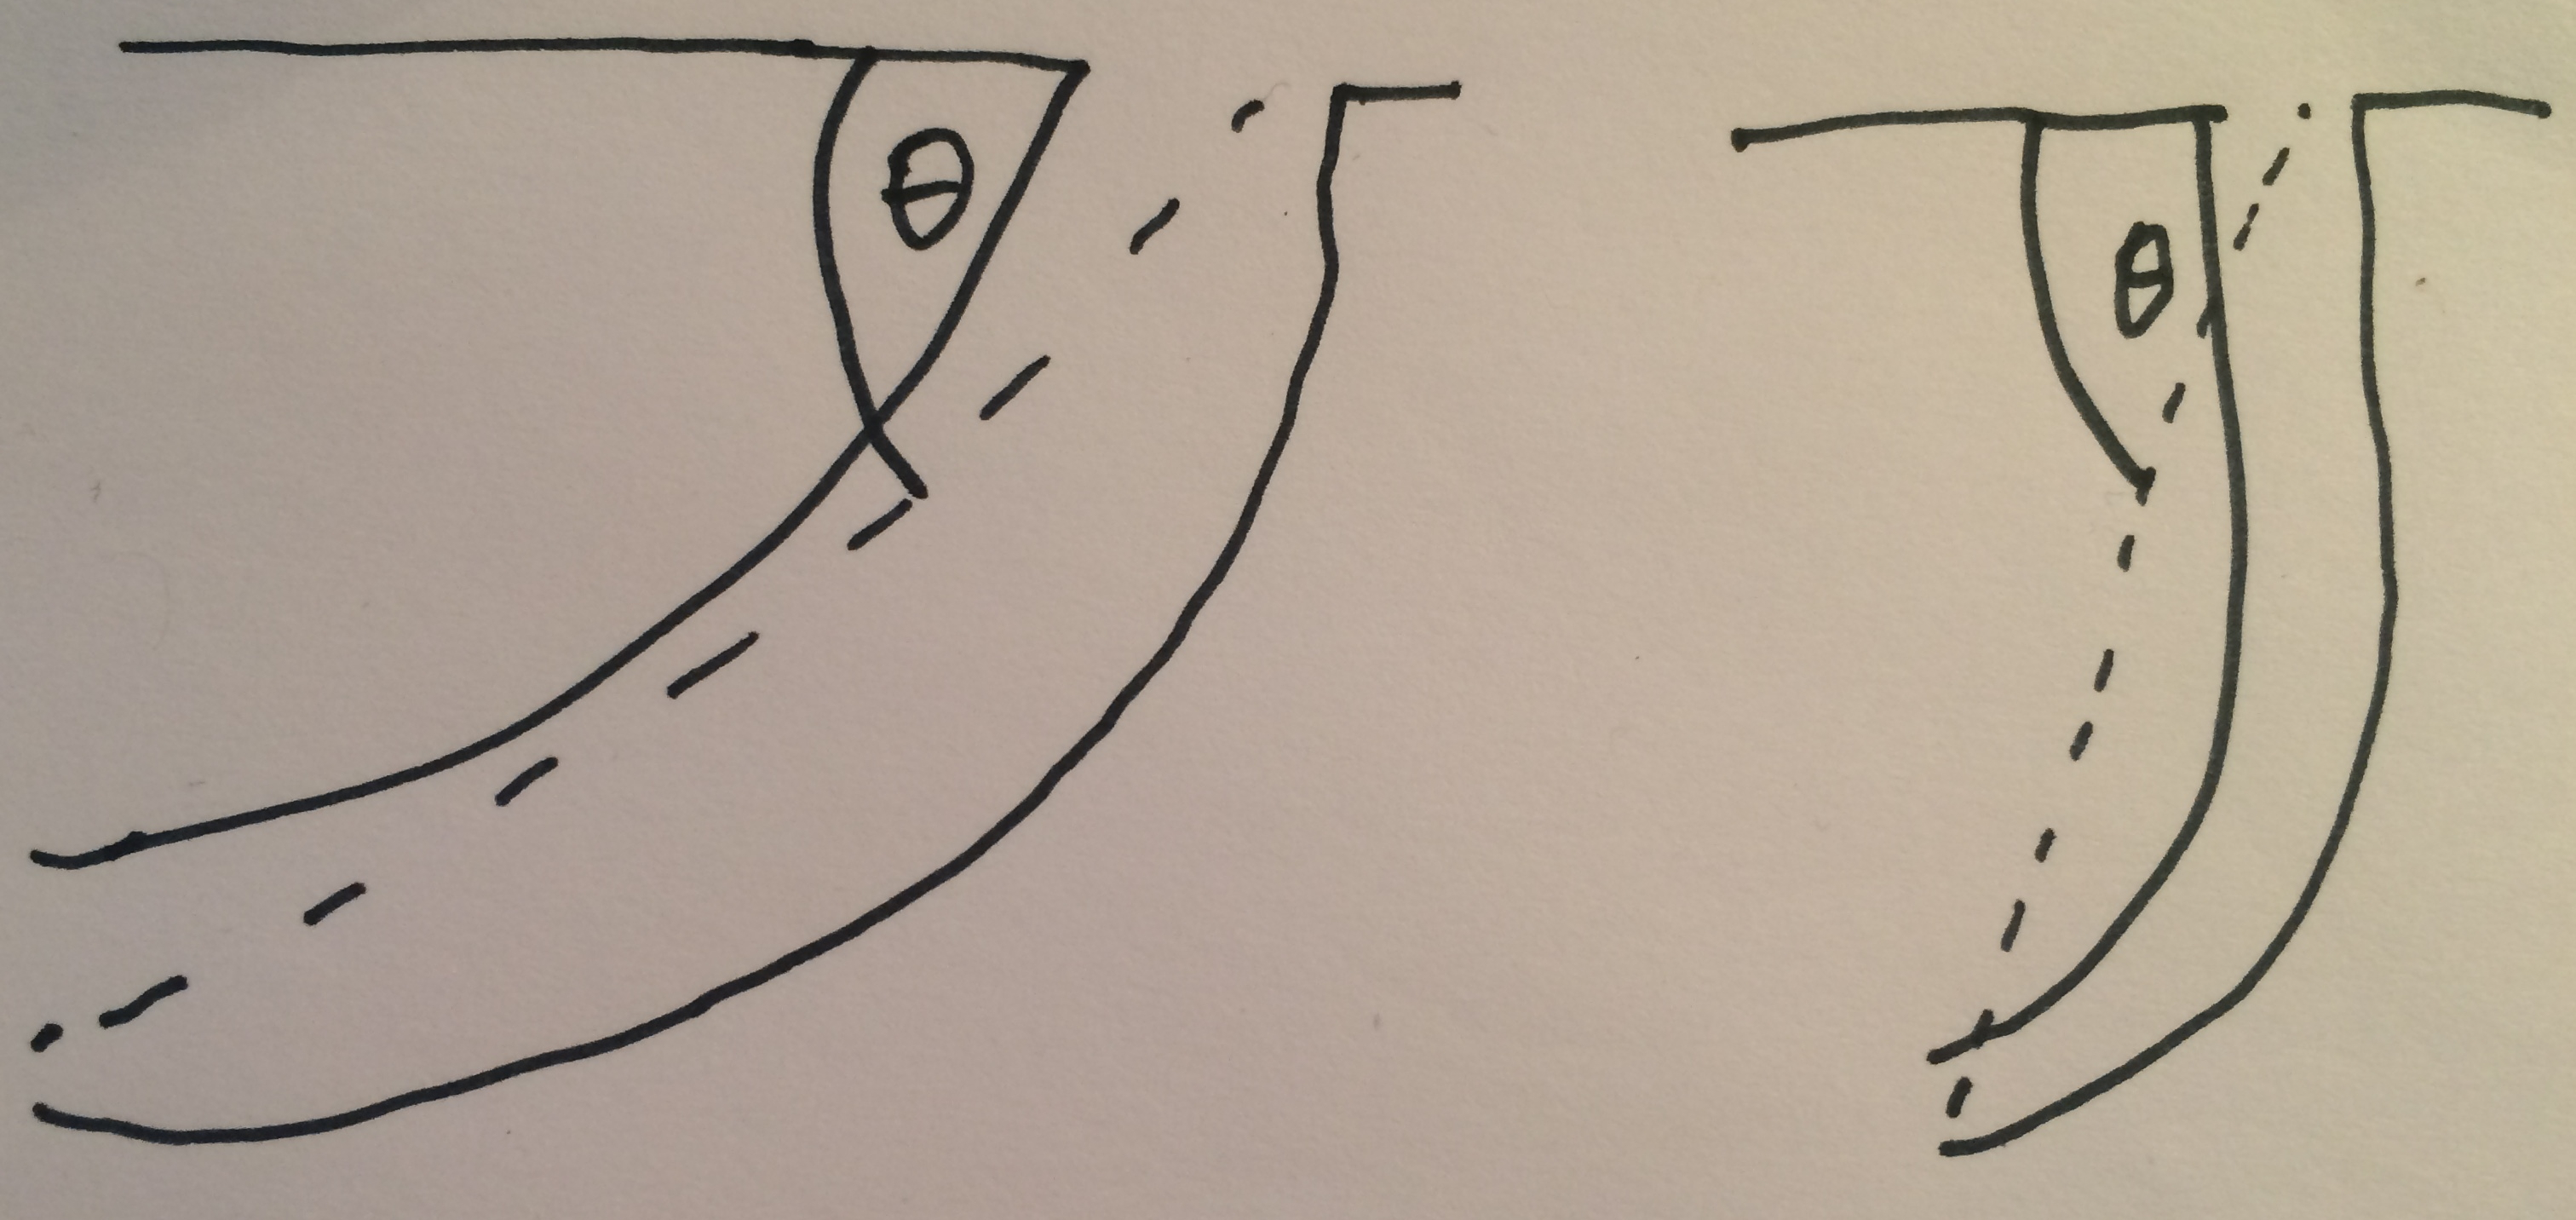
\includegraphics[width=\textwidth]{living_burrow_angle}
   	\caption{Burrow angle as defined by Endo \cite{endo2007}.}
   	\label{fig:living_burrow_angle}
   \end{figure}
   \begin{figure}[h]
   	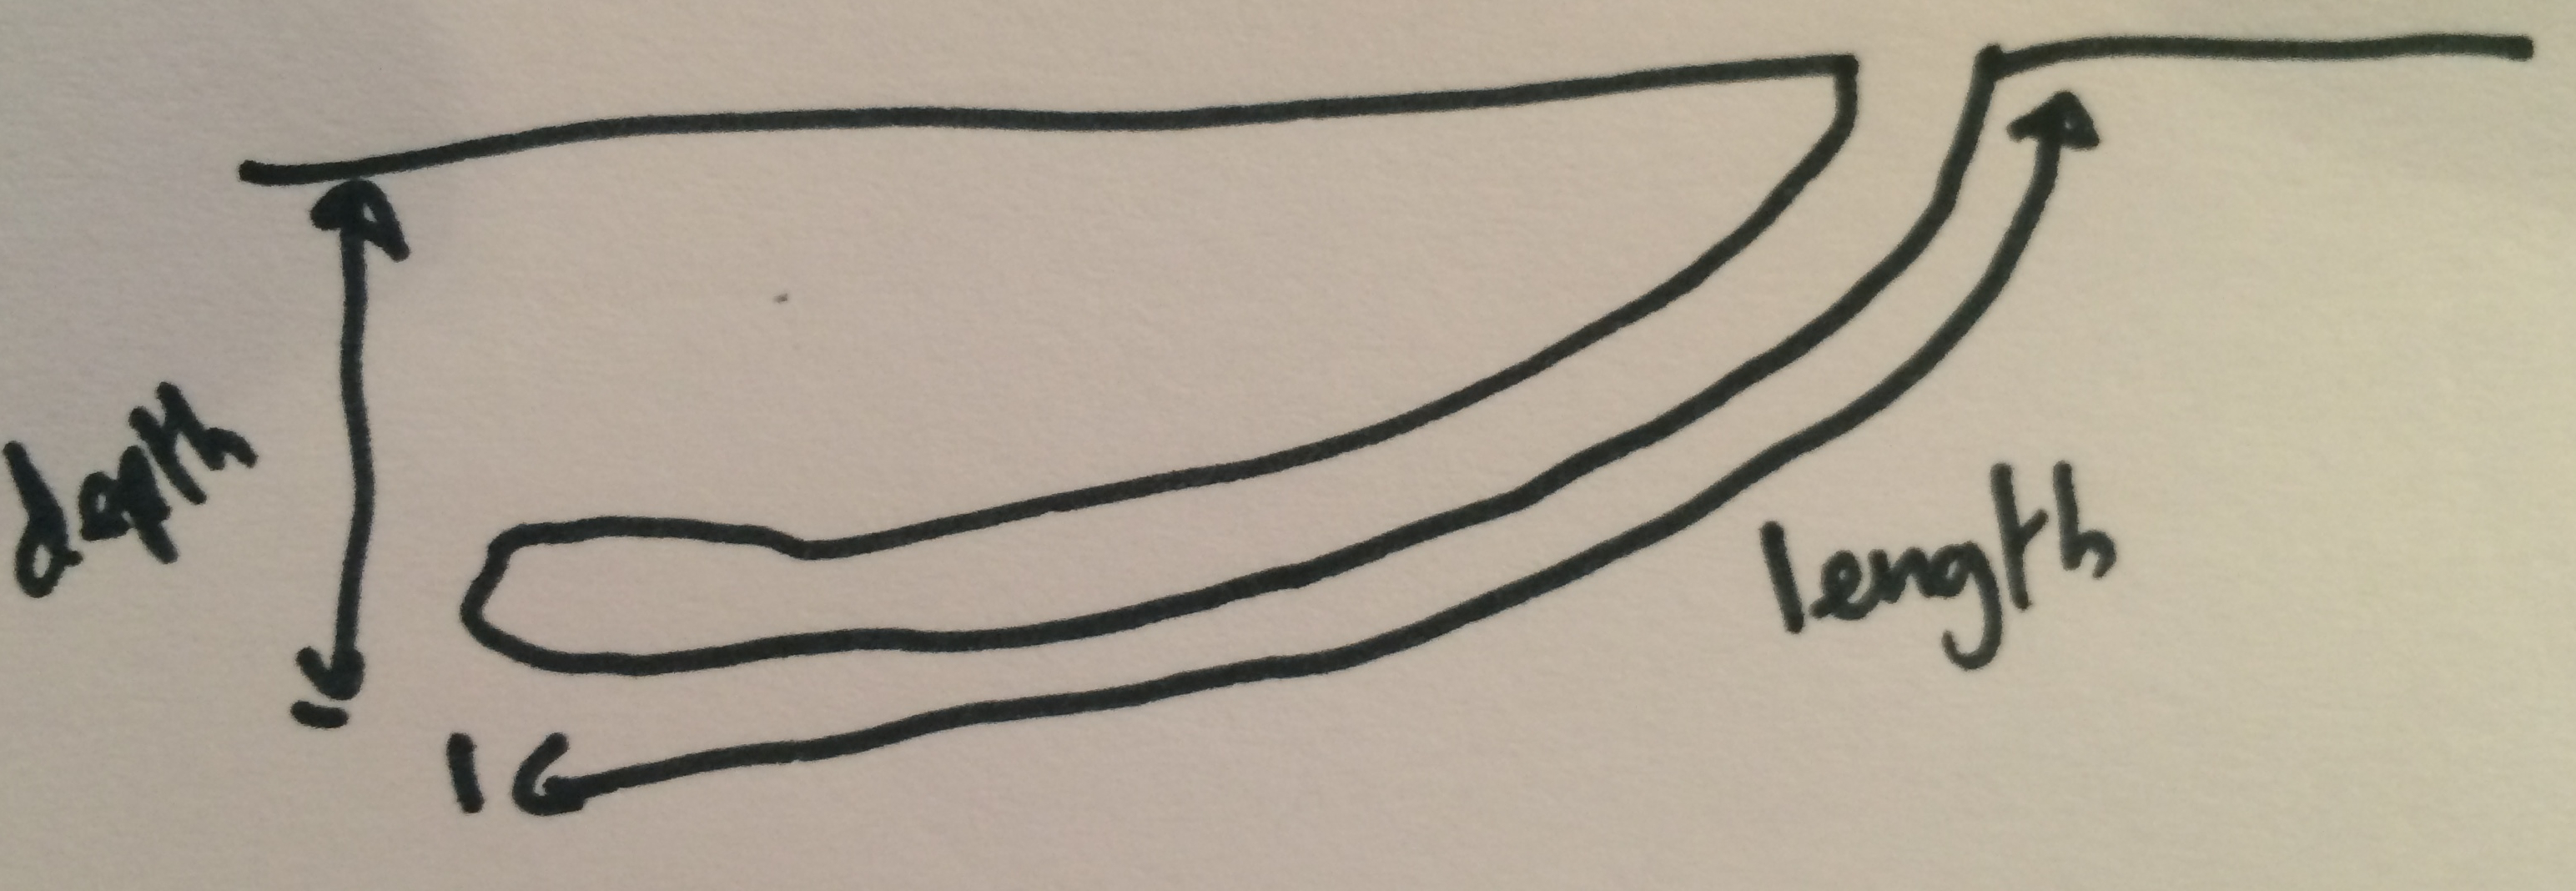
\includegraphics[width=\textwidth]{living_measurements}
   	\caption{Burrow measurements as defined by Endo \cite{endo2007}.}
   	\label{fig:living_measurements}
   \end{figure}
   \subsubsection{Horizontal burrows}
   Horizontal burrows may be used for feeding on creeping plants with shallow root systems \cite{endo2007}. Endo \cite{endo2007} found that the horizontal burrows of \textit{Gryllotalpa orientalis} had a number of openings (windows) that may act as traps for small arthropods. These arthropods enter the burrow system and may become prey for the mole cricket. Horizontal burrows may also provisde shelter from predators and act as routes to access potential mates \cite{endo2007}.
   \paragraph{Branch Points and Intersections}
   Branch points occur when a living burrow (either horizontal or vertical) forks. They are distinct from intersections which is where a horizontal and vertical tunnel meet.
   \paragraph{Escape Efficiency Index}
   An additional use of horizontal burrows is as an escape route from predators. Endo \cite{endo2008} proposes an escape efficiency index by dividing the total length of the horizontal burrows by the number of branching points in the horizontal tunnels (Equation ~\ref{eq:escape_efficiency_index}).
   \begin{equation}
   EE = \frac{\sum{Length\ of\ horizontal\ branches}}{Number\ of\ horizontal\ branch\ points}
   \label{eq:escape_efficiency_index}
   \end{equation}
   \paragraph{Fractal Dimension}
   Fractal dimension analysis of horizontal burrows has been studied by Endo \cite{endo2008}. The degree to which horizontal branching (leading to a higher fractal dimension) occurs in a given species may be closely linked to their foraging strategy. 

   \subsubsection{Vertical burrows}
   Vertical burrows may be used for feeding on plants (e.g. grasses and rushes) that have subterranean stems. It has been suggested that mole crickets may dig vertical burrows in pursuit of prey animals \cite{brandenburg2002}.
   \paragraph{}
   The depth of vertical burrows provides protection from predators and is used by mole crickets as a safe place for moulting and overwintering \cite{endo2007}.
   
   \subsubsection{Entrances}
   Entrances to the burrow are often concealed, and an individual burrow may have multiple entrances depending on the species. In \textit{Neoscapteriscus borelli} most burrows have a Y-shaped appearance due to the presence of two entrances \cite{brandenburg2002}.
   \paragraph{}
   Living burrow entrances should not be confused with the more elabotrate openings of the acoustic burrows of the males, which are predominantly shaped to improve transmission of the male's courtship song.
   
   \subsubsection{Egg Chambers}
   Egg chambers are generally sealed to prevent predators from entering the chapter. They may be located besides a horizontal burrow \cite{endo2007}.
   
   
   
   \subsection{Acoustic Burrows}
   The acoustic burrows of \textit{Gryllotalpa} (Figure ~\ref{fig:acoustic_overview}-~\ref{fig:acoustic_overview_lateral}) consist of an acoustically tuned bulb and between one and four exponential horns (see species accounts). The openings of the horns of at least one species (\textit{Gryllotalpa major}) vary in shape \cite{hill2006}. The bulb also has an exit tunnel leading away from the horns, which connects to the main burrow network. This provides protection to the male and his mate once she has located his burrow, or an escape route should his song inadvertently attract a predator.
   \begin{figure}[h]
   	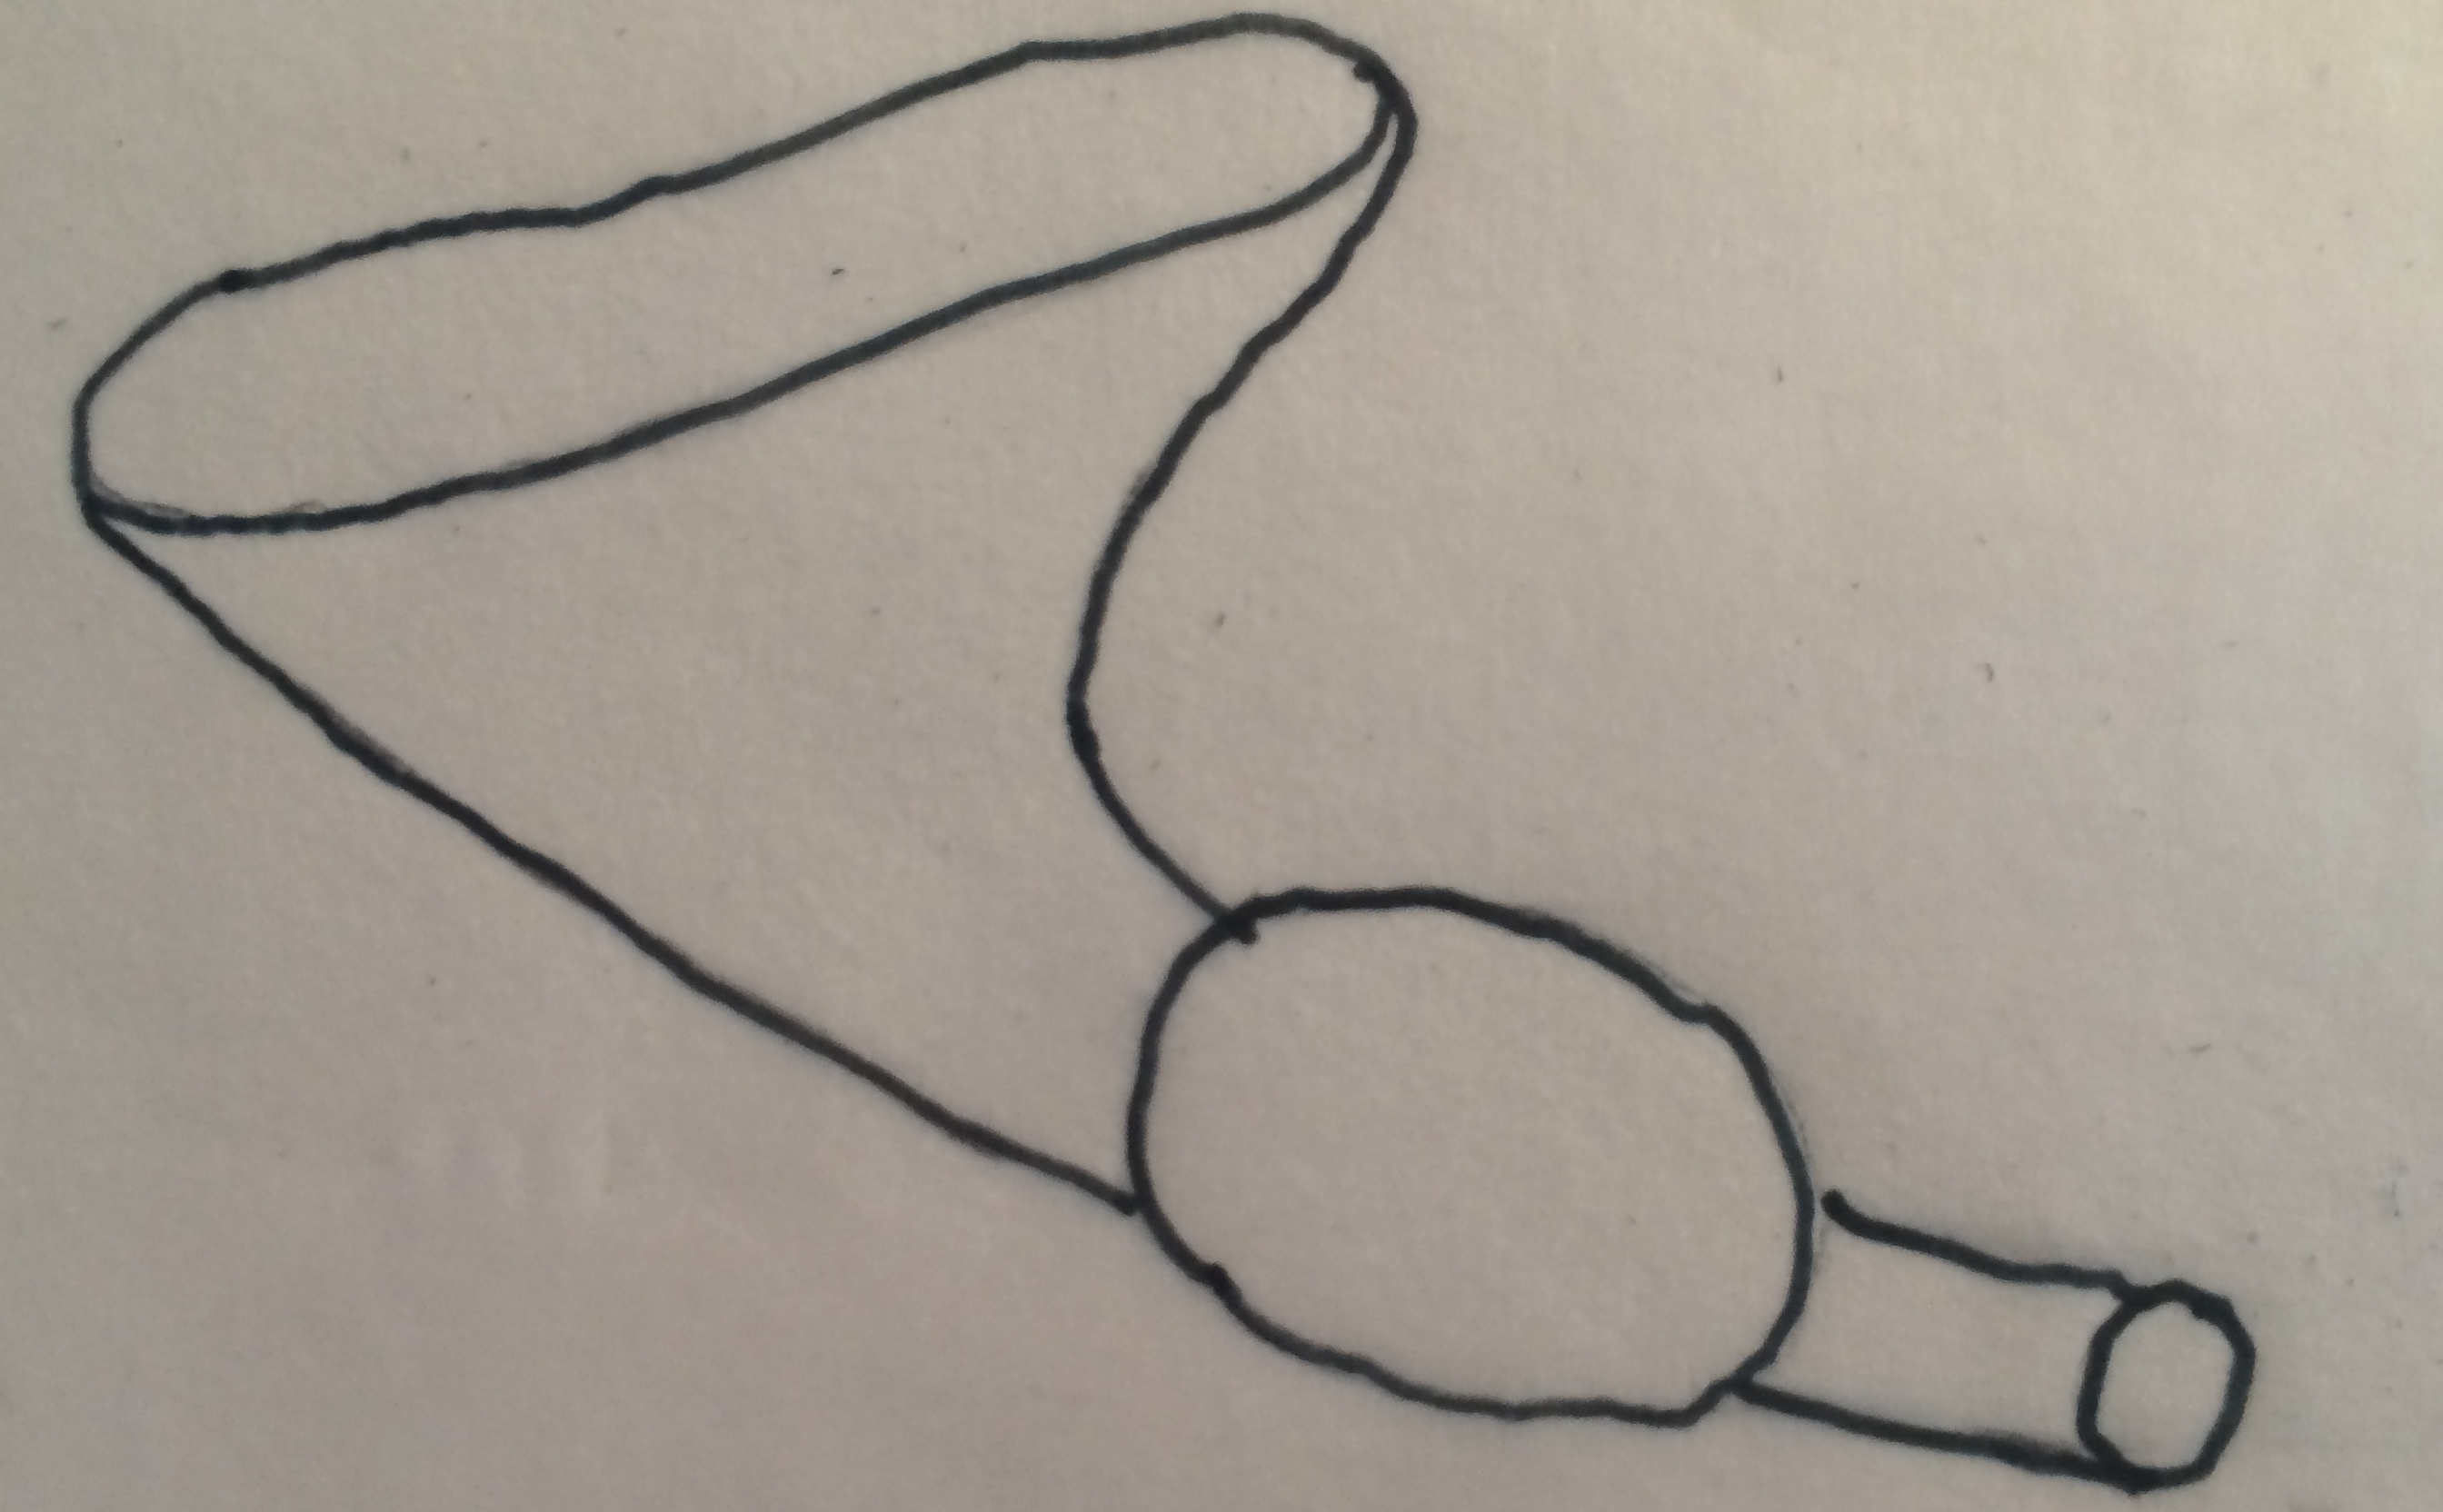
\includegraphics[width=\textwidth]{acoustic_overview}
   	\caption{Overview of an acoustic burrow of \textit{Gryllotalpa major} showing the exponential horn and bulb. Based on \cite{walker1990}.}
   	\label{fig:acoustic_overview}
   \end{figure}
   \begin{figure}[h]
   	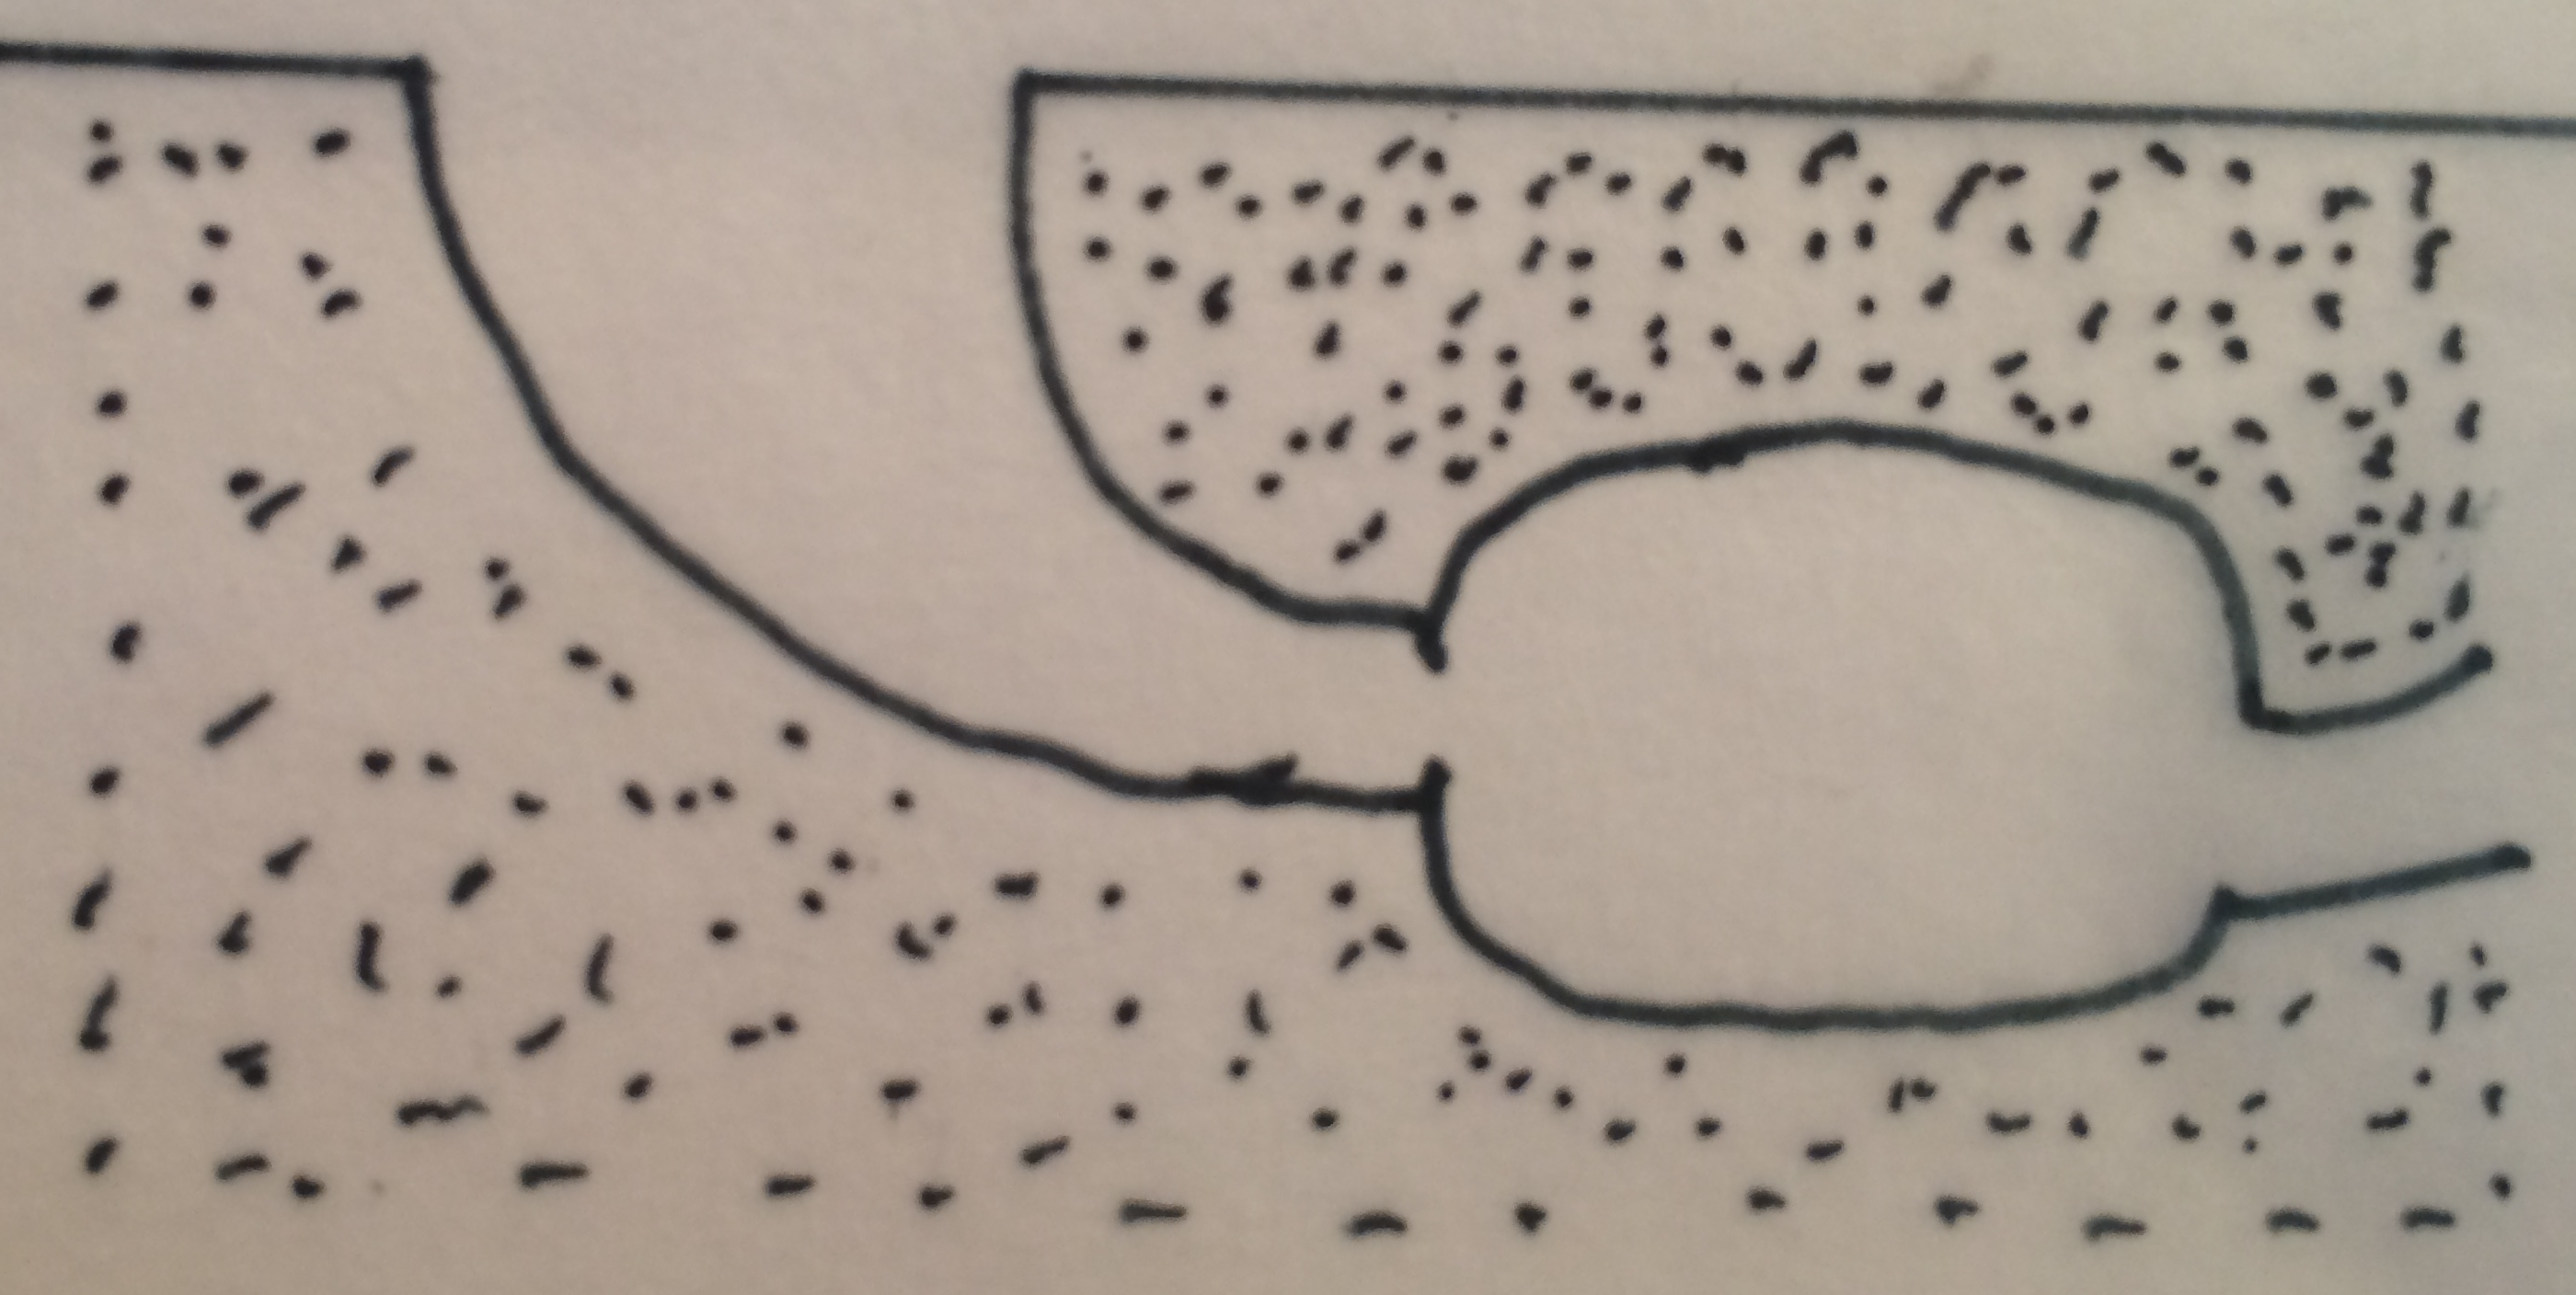
\includegraphics[width=\textwidth]{acoustic_overview_lateral}
   	\caption{Lateral view of an acoustic burrow of \textit{Gryllotalpa major} showing the exponential horn and bulb. Based on \cite{walker1990}.}
   	\label{fig:acoustic_overview_lateral}
   \end{figure}
   
   \subsubsection{Orientation}
   When describing the shape of the horn opening (see below) it is useful to arbitrarily define an orientation for the burrow system. The anterior end of the acoustic burrow is defined as the end with the horn opening. This terminology is currently only used to describe the arrangement of horns when they occur in more than one row.
   
   \subsubsection{Offset horn}
   Hill et al \cite{hill2006} differentiate between 'slit' and 'L-shaped' burrows of \textit{Gryllotalpa major} that has a single highly elliptical horn opening. The actual horn opening of these two burrow forms are however the same. The difference between these two burrow forms is actually an offsetting of the horn from the normal plane of the bulb, perhaps due to soil conditions.
   
   The term offset is used here as a measure of the asymmetry of the burrow (Figure ~\ref{fig:acoustic_horn_offset}).
   
   \begin{figure}[h]
   	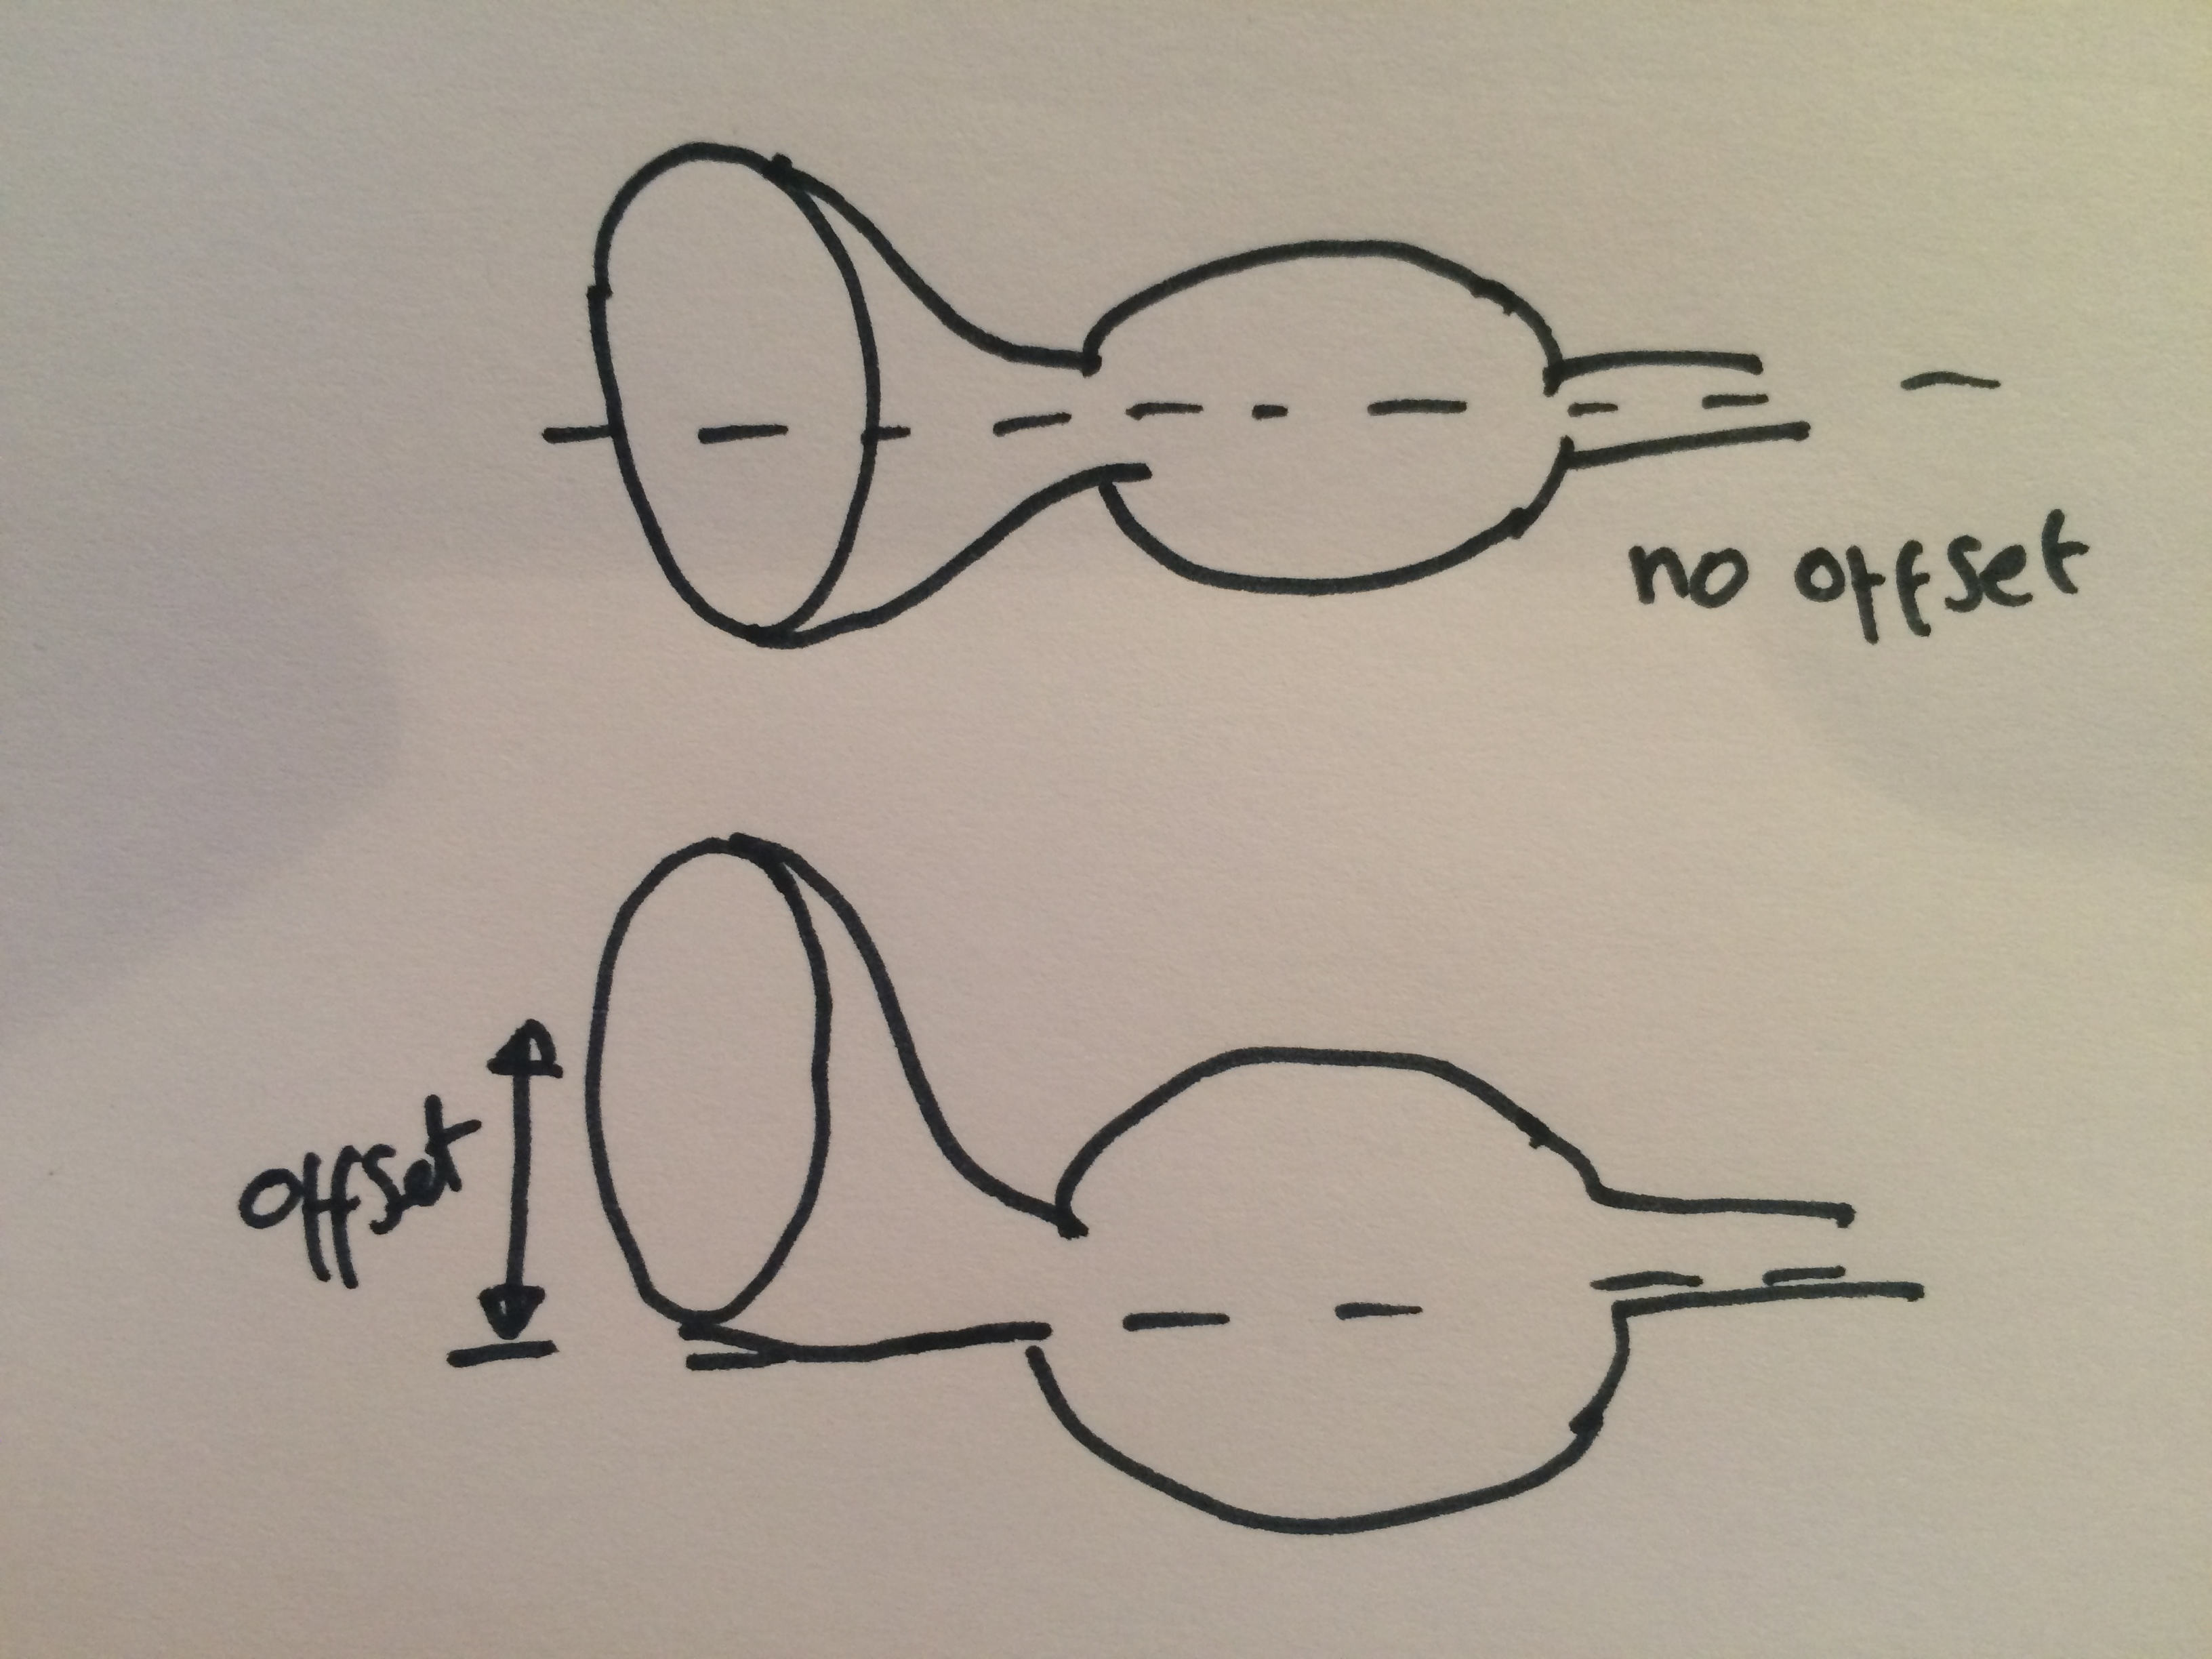
\includegraphics[width=\textwidth]{acoustic_horn_offset}
   	\caption{}
   	\label{fig:acoustic_horn_offset}
   \end{figure}
   
   \subsubsection{Horn number and arrangement}
   The horn number is defined simply as the number of horns present in the burrow. The naming of individual horns is defined simply by number in the case of the horns being approximately along a straight line (Figure ~\ref{fig:acoustic_horn_number}).
   \paragraph{}
   In the case of \textit{Gryllotalpa australis} where the burrow consists of four horns arranged in two rows the rows are identified as anterior and posterior using the orientation of the burrow, and then numbered individually.
   \paragraph{}
   The use of a numerical system, or when needed a numerical system with a named row is used rather a more vernacular system (left, right, centre) to allow for flexibility in describing as yet unknown burrows.
   
   \begin{figure}[h]
   	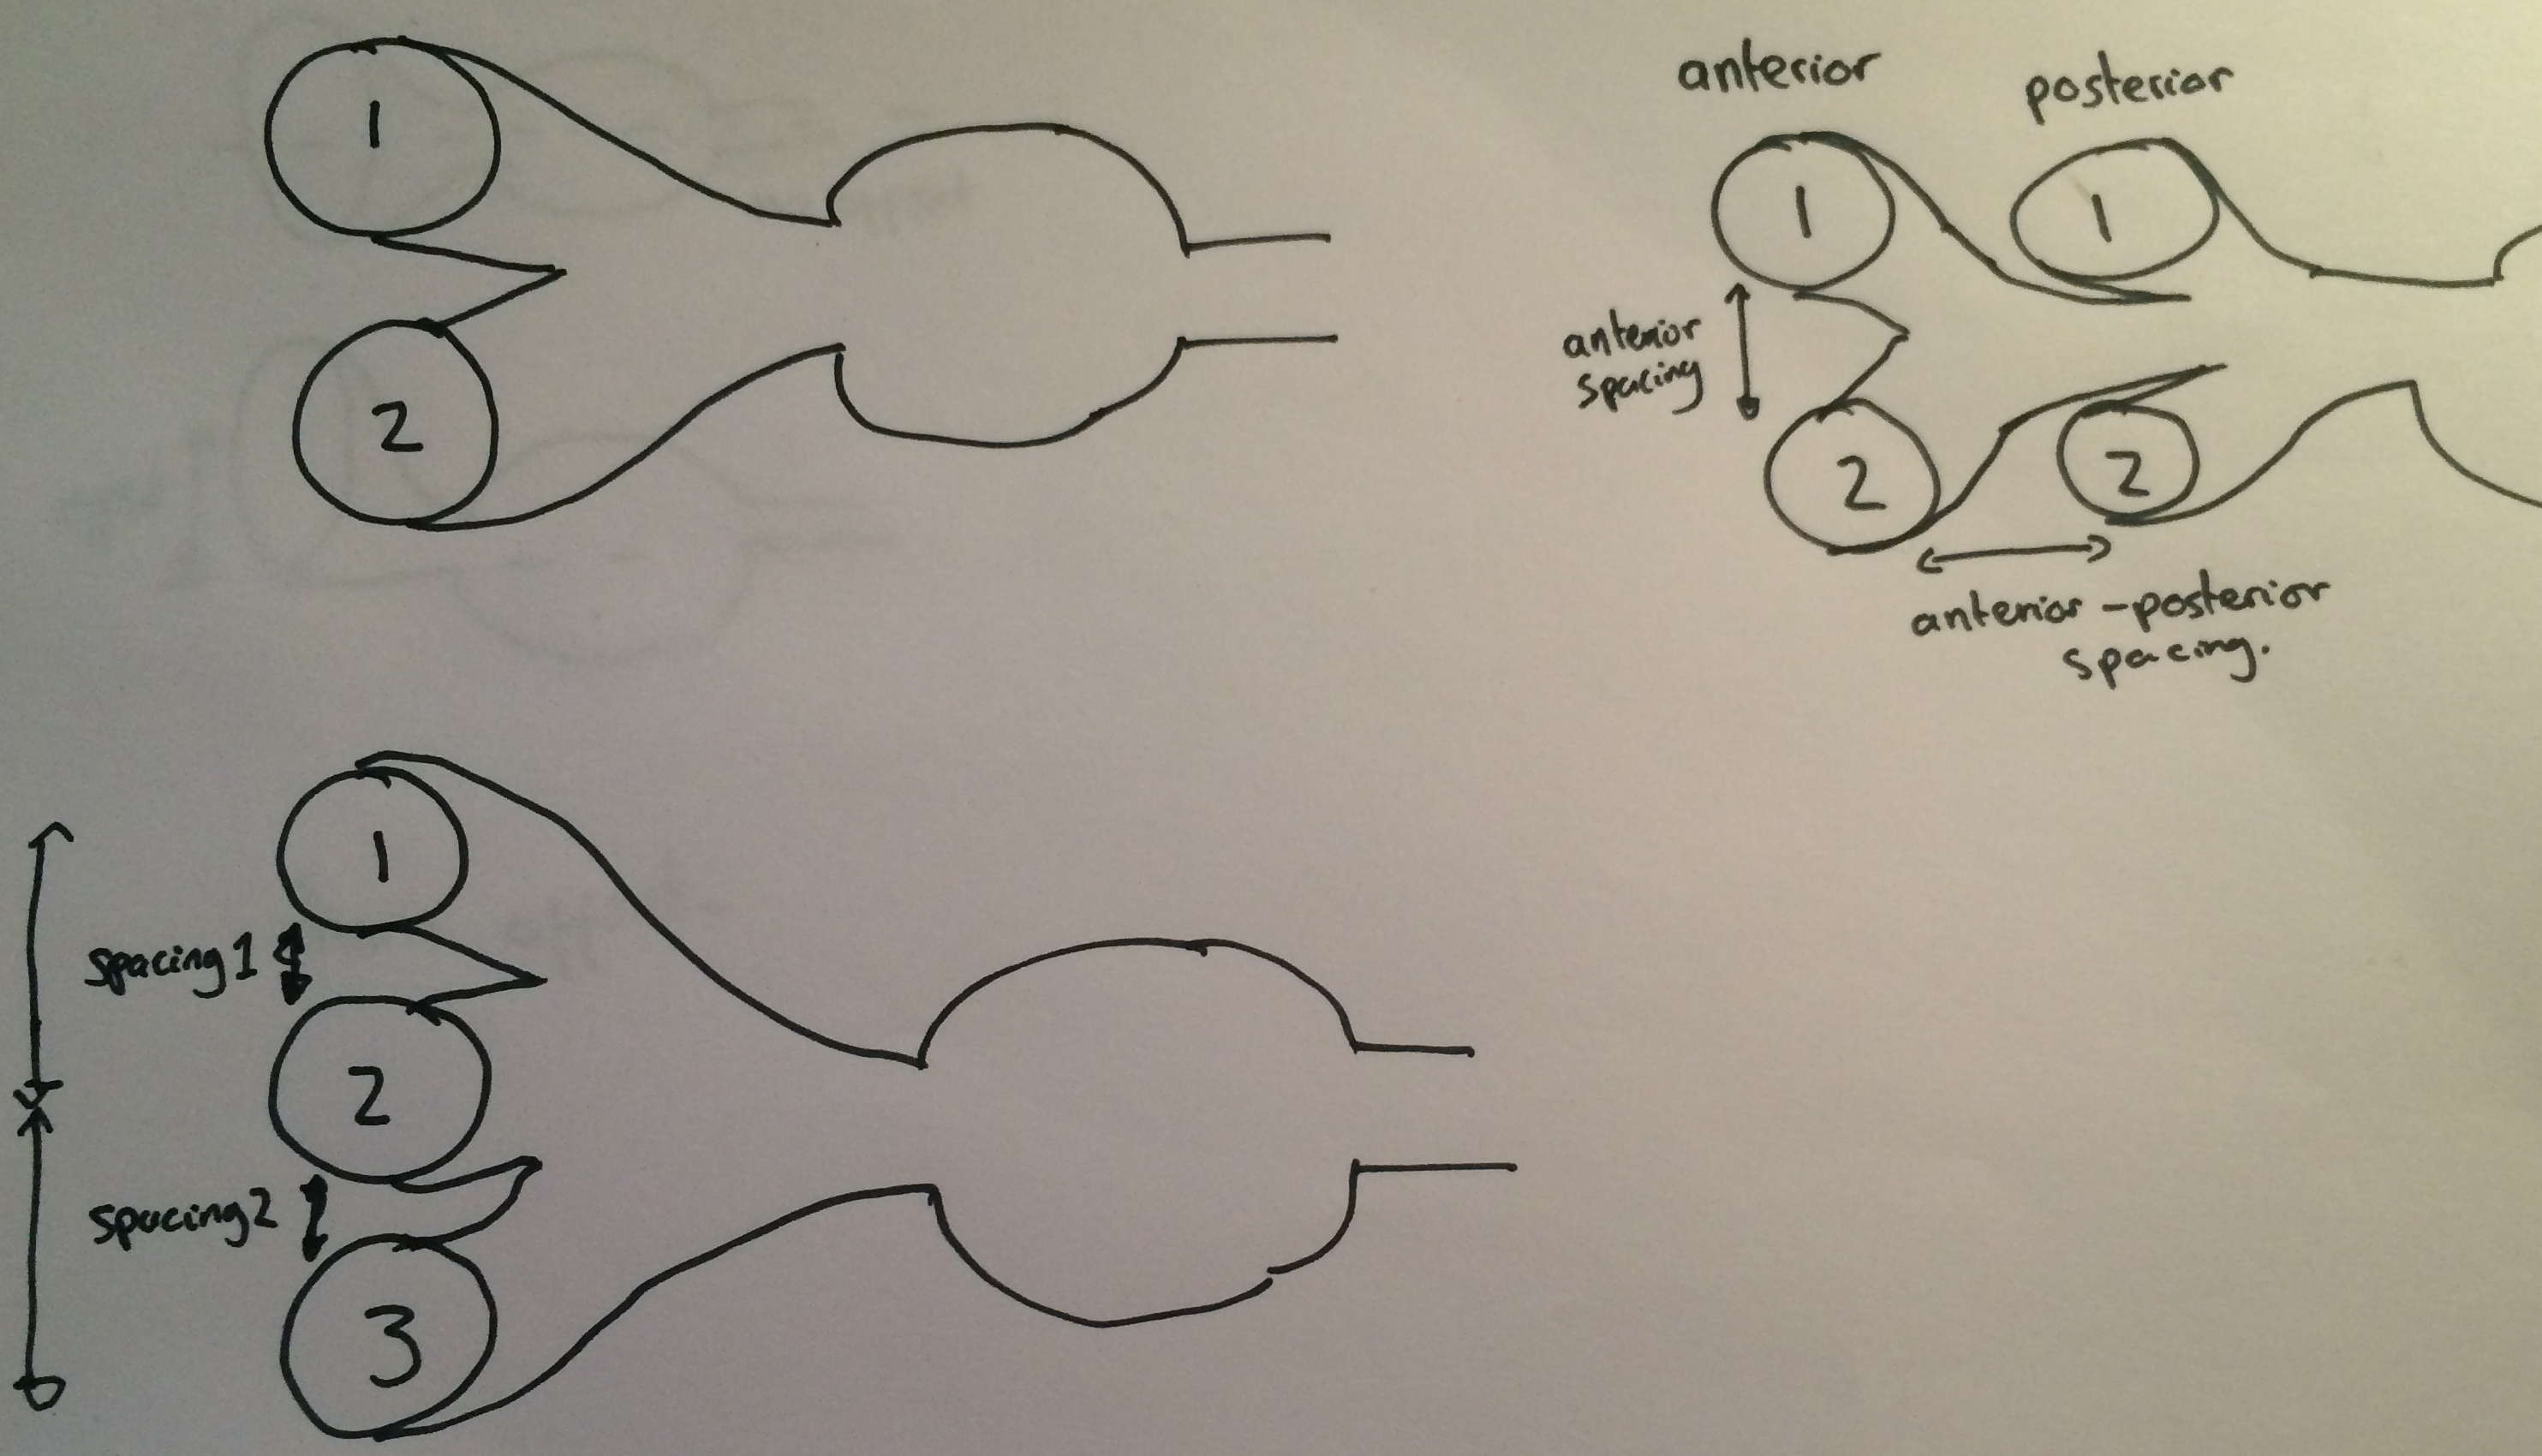
\includegraphics[width=\textwidth]{acoustic_horn_number}
   	\caption{Arrangement and identification of horns and horn openings.}
   	\label{fig:acoustic_horn_number}
   \end{figure}
   
   \subsubsection{Horn Opening}
   In their study of the burrows of \textit{Gryllotalpa major} Walker \& Figg \cite{walker1990} transpose the axes of width and length between the bulb and horn opening, a practise followed by \cite{jafari2015}. I propose here to switch the opening length and opening width (sensu \cite{walker1990}) in order to provide a consistent system, with all length measurements along the same axis (Figure ~\ref{fig:acoustic_measurements}).
   \paragraph{Horn length}
   The horn length is taken  by previous authors to be the distance of an imagined wire following the centre of the horn from the throat to the opening. It is not clear whether \cite{jafari2015} followed this procedure. As measurement of this property is practically difficult it may be better to measure the smallest horn length (from the top of the throat to the rear of the opening) and largest horn length (from the bottom of the throat to the front of the horn).
   \paragraph{Opening shape}
   The opening shape terminology used by Hill et al \cite{hill2006} is adopted with modifications. 'Oval' is added to account for the oval horn openings of \textit{Gryllotalpa vineae} (and others), and L-shaped is dropped as this is not a feature of the horn opening, and is covered above in Offset Bulbs. Opening shapes are shown in Figure ~\ref{fig:acoustic_opening_shape}.
   \paragraph{Eccentricity of oval openings}
   TODO: Orientation
   \begin{figure}[h]
   	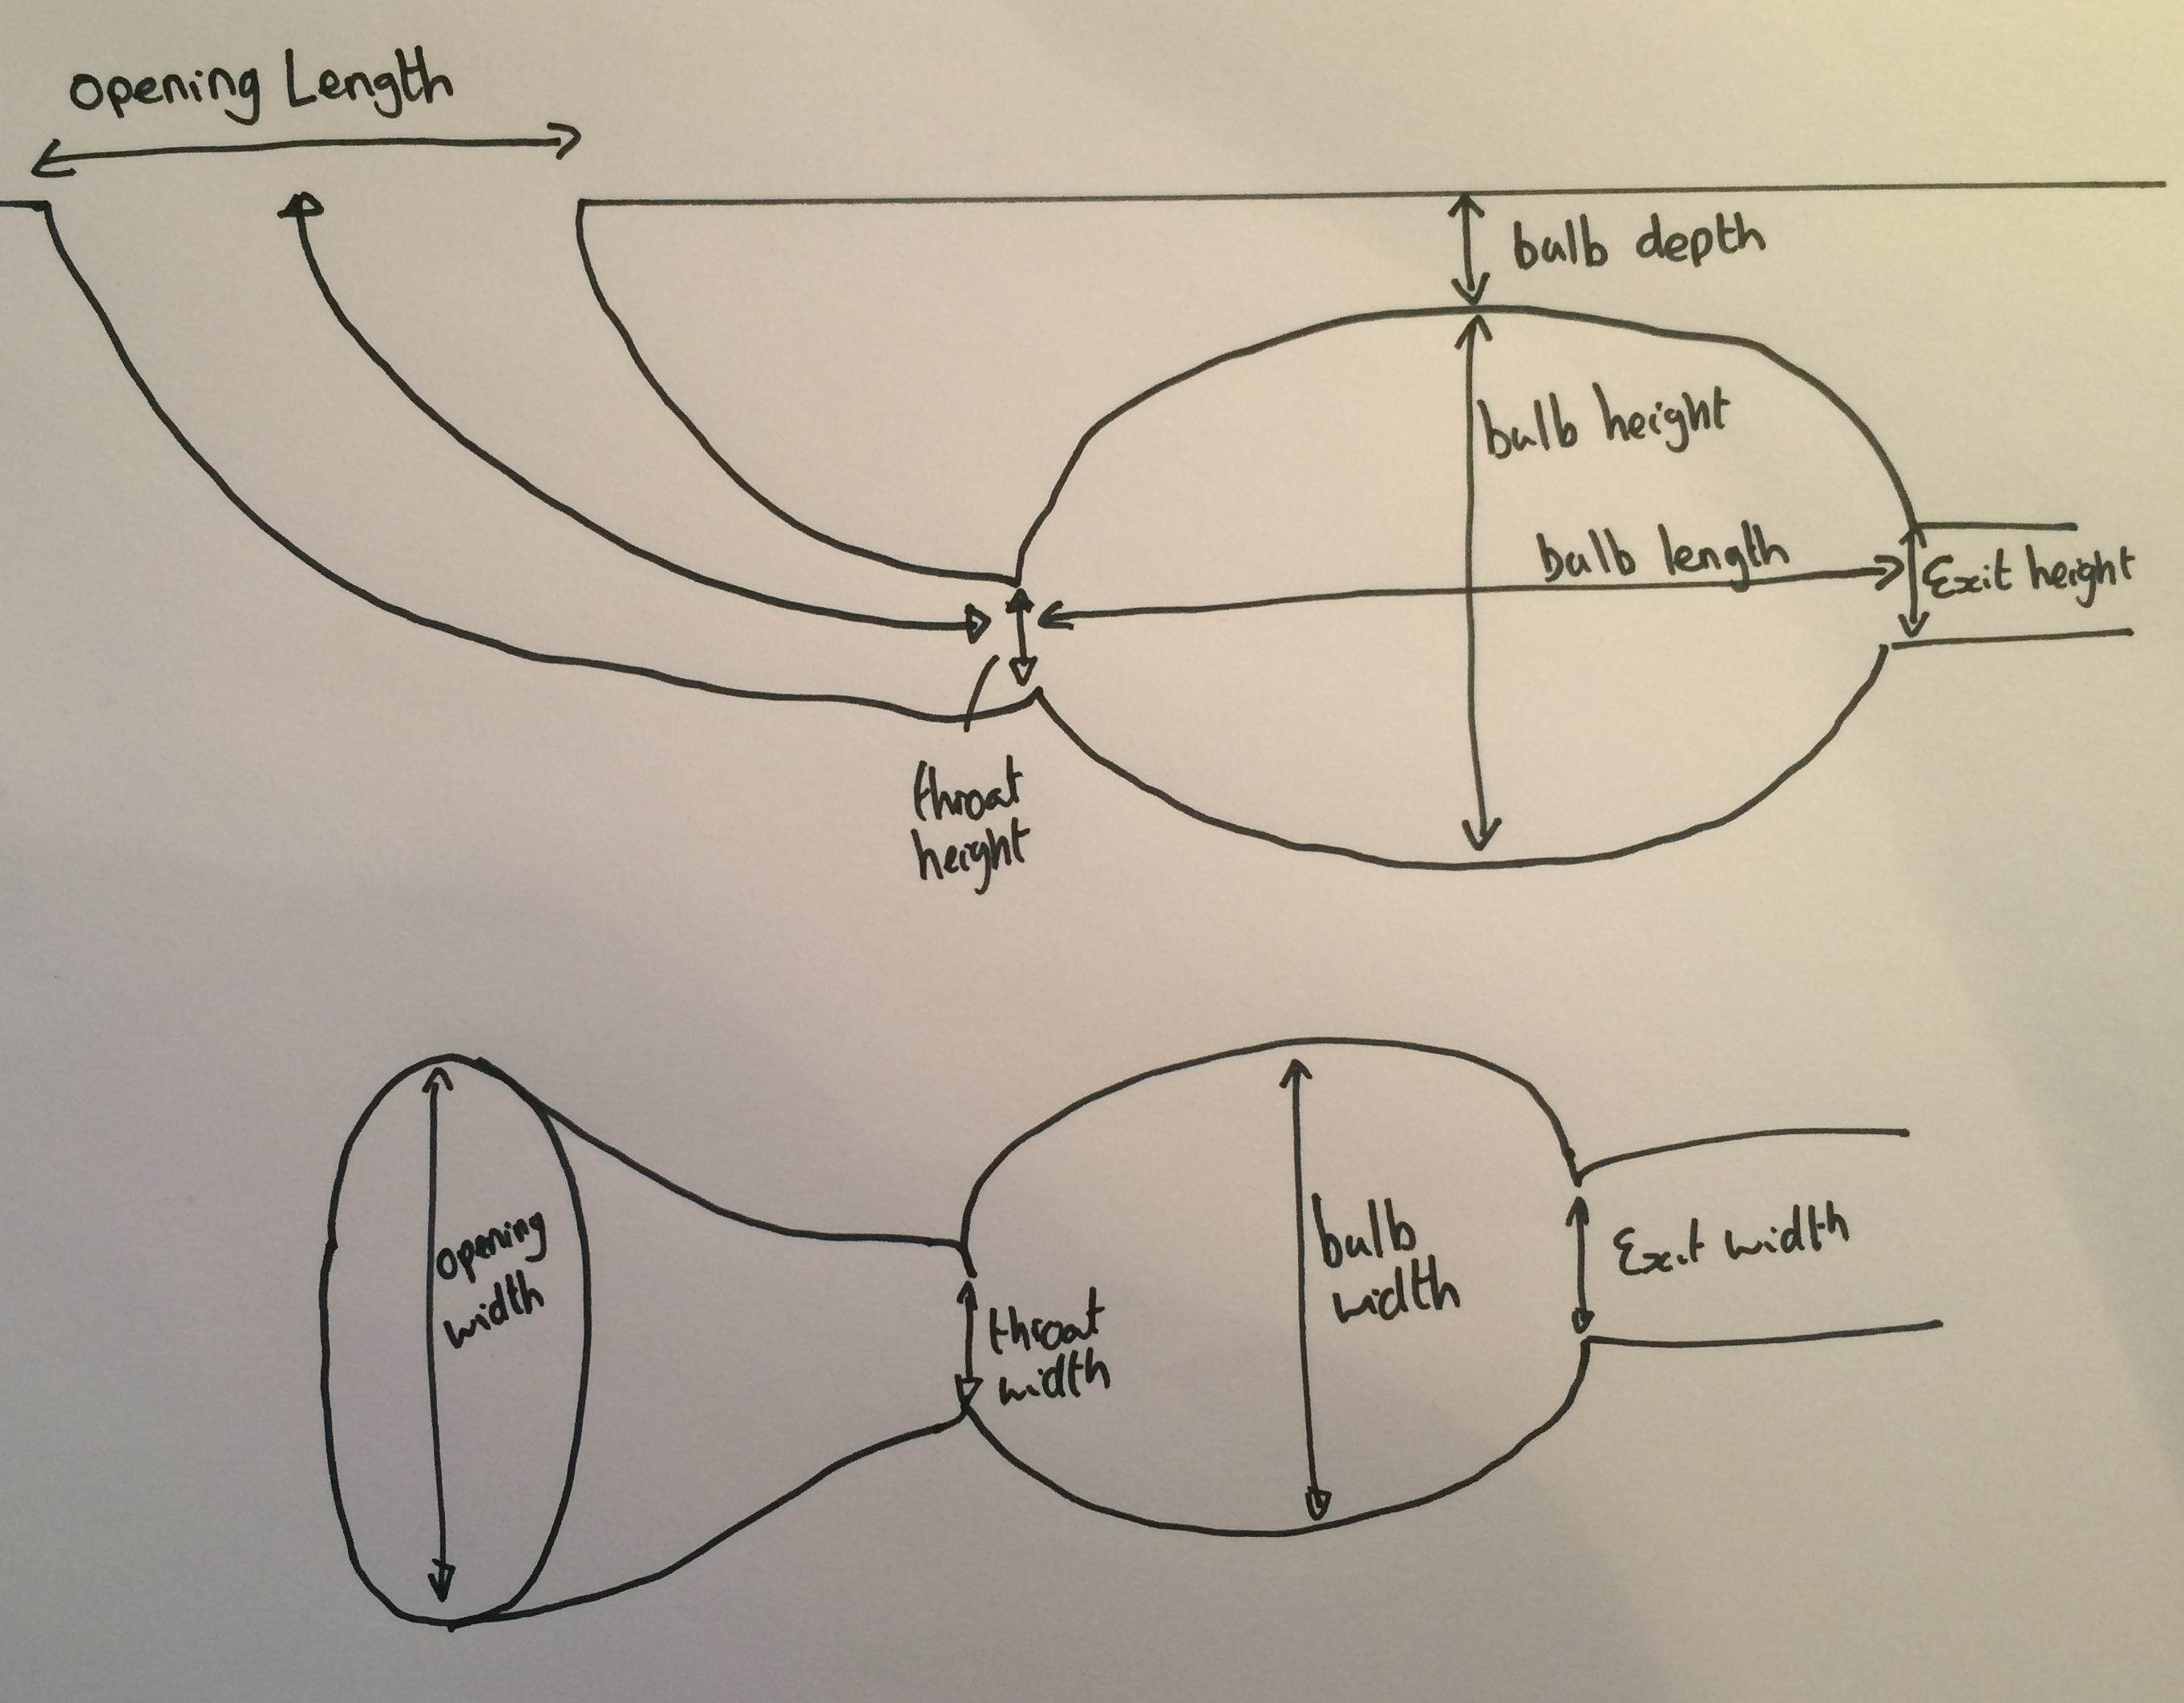
\includegraphics[width=\textwidth]{acoustic_measurements}
   	\caption{}
   	\label{fig:acoustic_measurements}
   \end{figure}
   
   \begin{figure}[h]
   	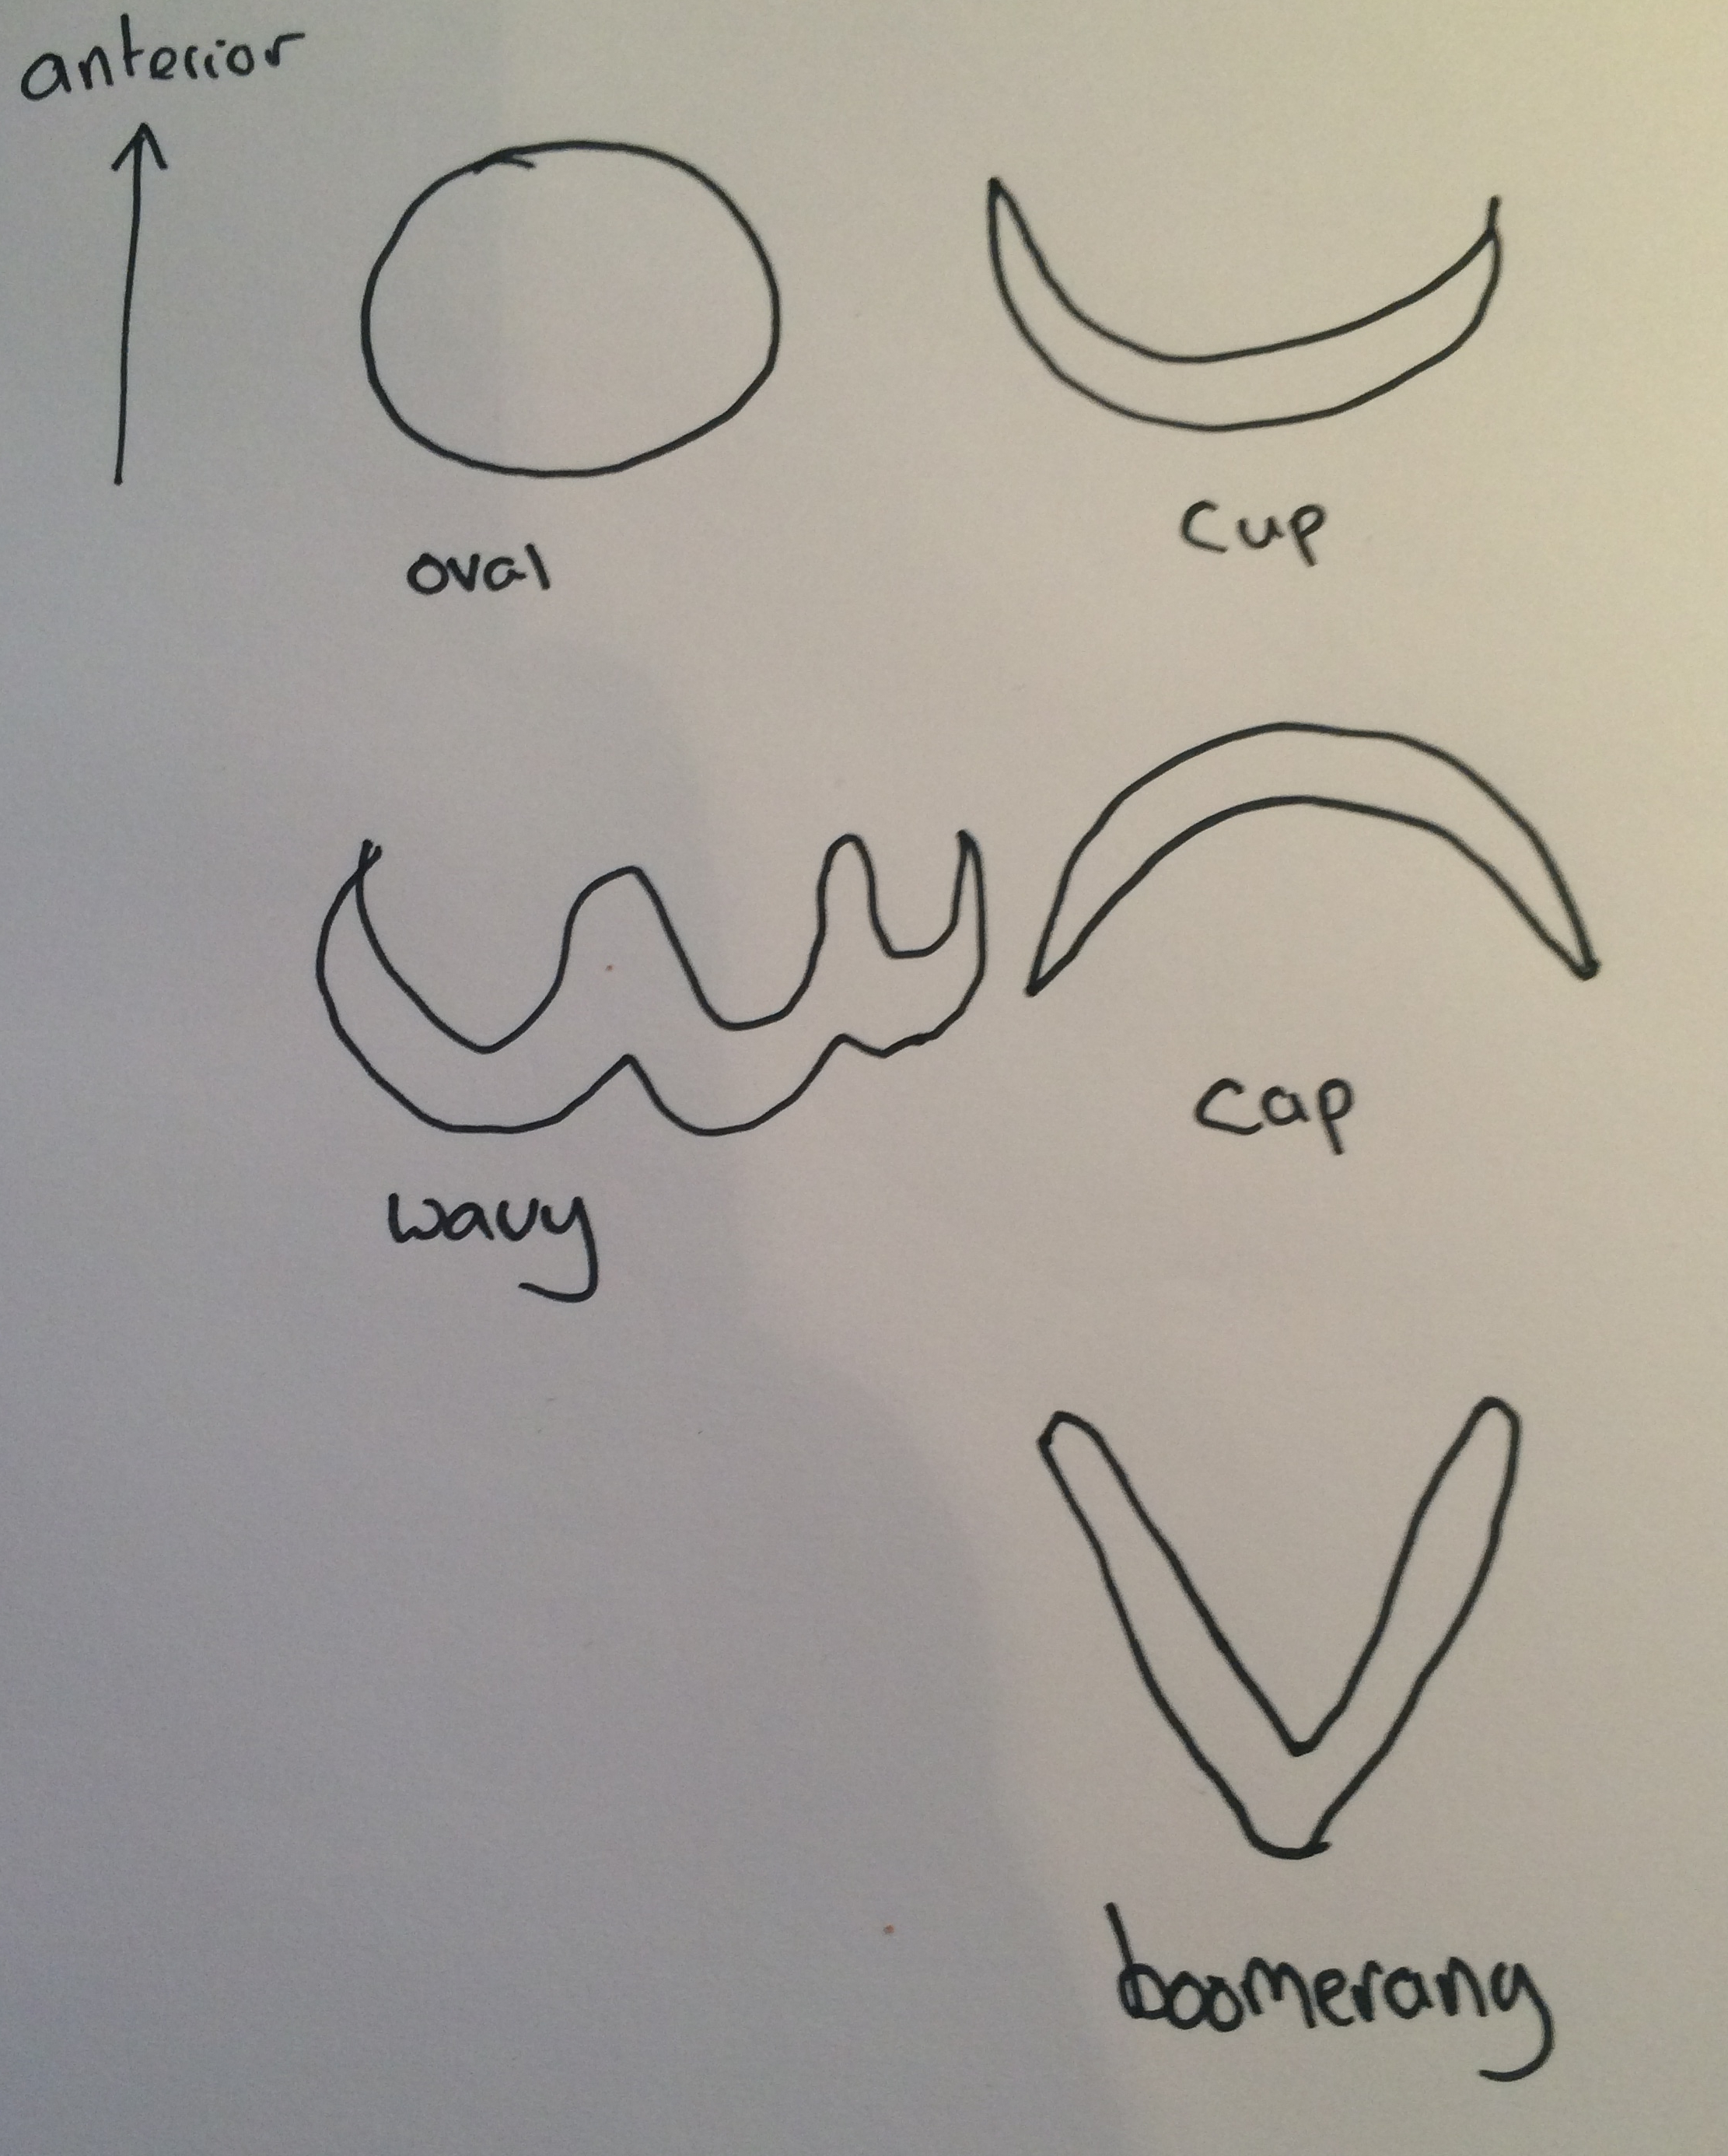
\includegraphics[width=\textwidth]{acoustic_opening_shape}
   	\caption{}
   	\label{fig:acoustic_opening_shape}
   \end{figure}
   
   \subsubsection{Horn spacing}
   Along with the dimensions of the horn openings, the spacing between openings may have an impact on the acoustic properties of the overall acoustic burrow system. For an acoustic burrow with two horns the horn spacing is the distance between the midpoints of the two horn openings. For acoustic burrows with three or more horn openings the horn spacings are a series of measurements between the midpoints of horn openings. In the case where there are two rows of horn openings measurements should be taken of the anterior spacing, the anterior-posterior spacing and the posterior spacing (Figure ~\ref{fig:acoustic_horn_number}).
   
   \subsubsection{Bulb}
   All reports of acoustic burrows in the literature have a single bulb. A cast of \textit{Gryllotalpa gryllotalpa} held in the NHM (NHMUK010211142) however could be considered to have two bulbs (FIG). For now the specimen is treated as having a single bulb.
   
   \subsubsection{Throat and exit}
   The acoustic burrow of mole crickets has two constrictions, one between the horn(s) and the bulb, and another between the bulb and the exit to he main tunnel system. I have followed the terminology used by \cite{jafari2015}, with the constriction between the horn and bulb being the 'throat' and the constriction between the bulb and the exit tunnel(s) being the 'exit'.
   
   \paragraph{}
   While some authors have measured the height and width of the constrictions separately (cite{jafari2015}) others have only specified a single diameter measurement (\cite{kavanagh1989}). 
   
   \subsubsection{Exit number and orientation}
   Previous publications on the morphology of acoustic burrows have shown the bulb to have two openings - one to the horn system and another, the exit tunnel, that links to the mole crickets living burrows. One burrow cast in the Natural History Museum (NHMUK010211180) however has two distinct exit tunnels (Figure ~\ref{fig:acoustic_two_exit}). This is likely to be caused by the cricket constructing the acoustic burrow at a point along an existing horizontal burrow, rather than at its terminus.  Exit tunnels are numbered in clockwise series from the horn opening. The exit angle is defined as the angle between the horn opening and the exit tunnel under consideration (Figure ~\ref{fig:acoustic_exit_angle}).
   
   \subsubsection{Turn around}
   Nickerson et al \cite{nickerson1979} show that the burrows of \textit{Neoscapteriscus} have an additional chamber to the bulb that appears to allow the insect to turn around while within the acoustic burrow complex (presumably to allow it to turn around into singing position after entering the acoustic burrow from the living burrow system).
   
   \begin{figure}[h]
   	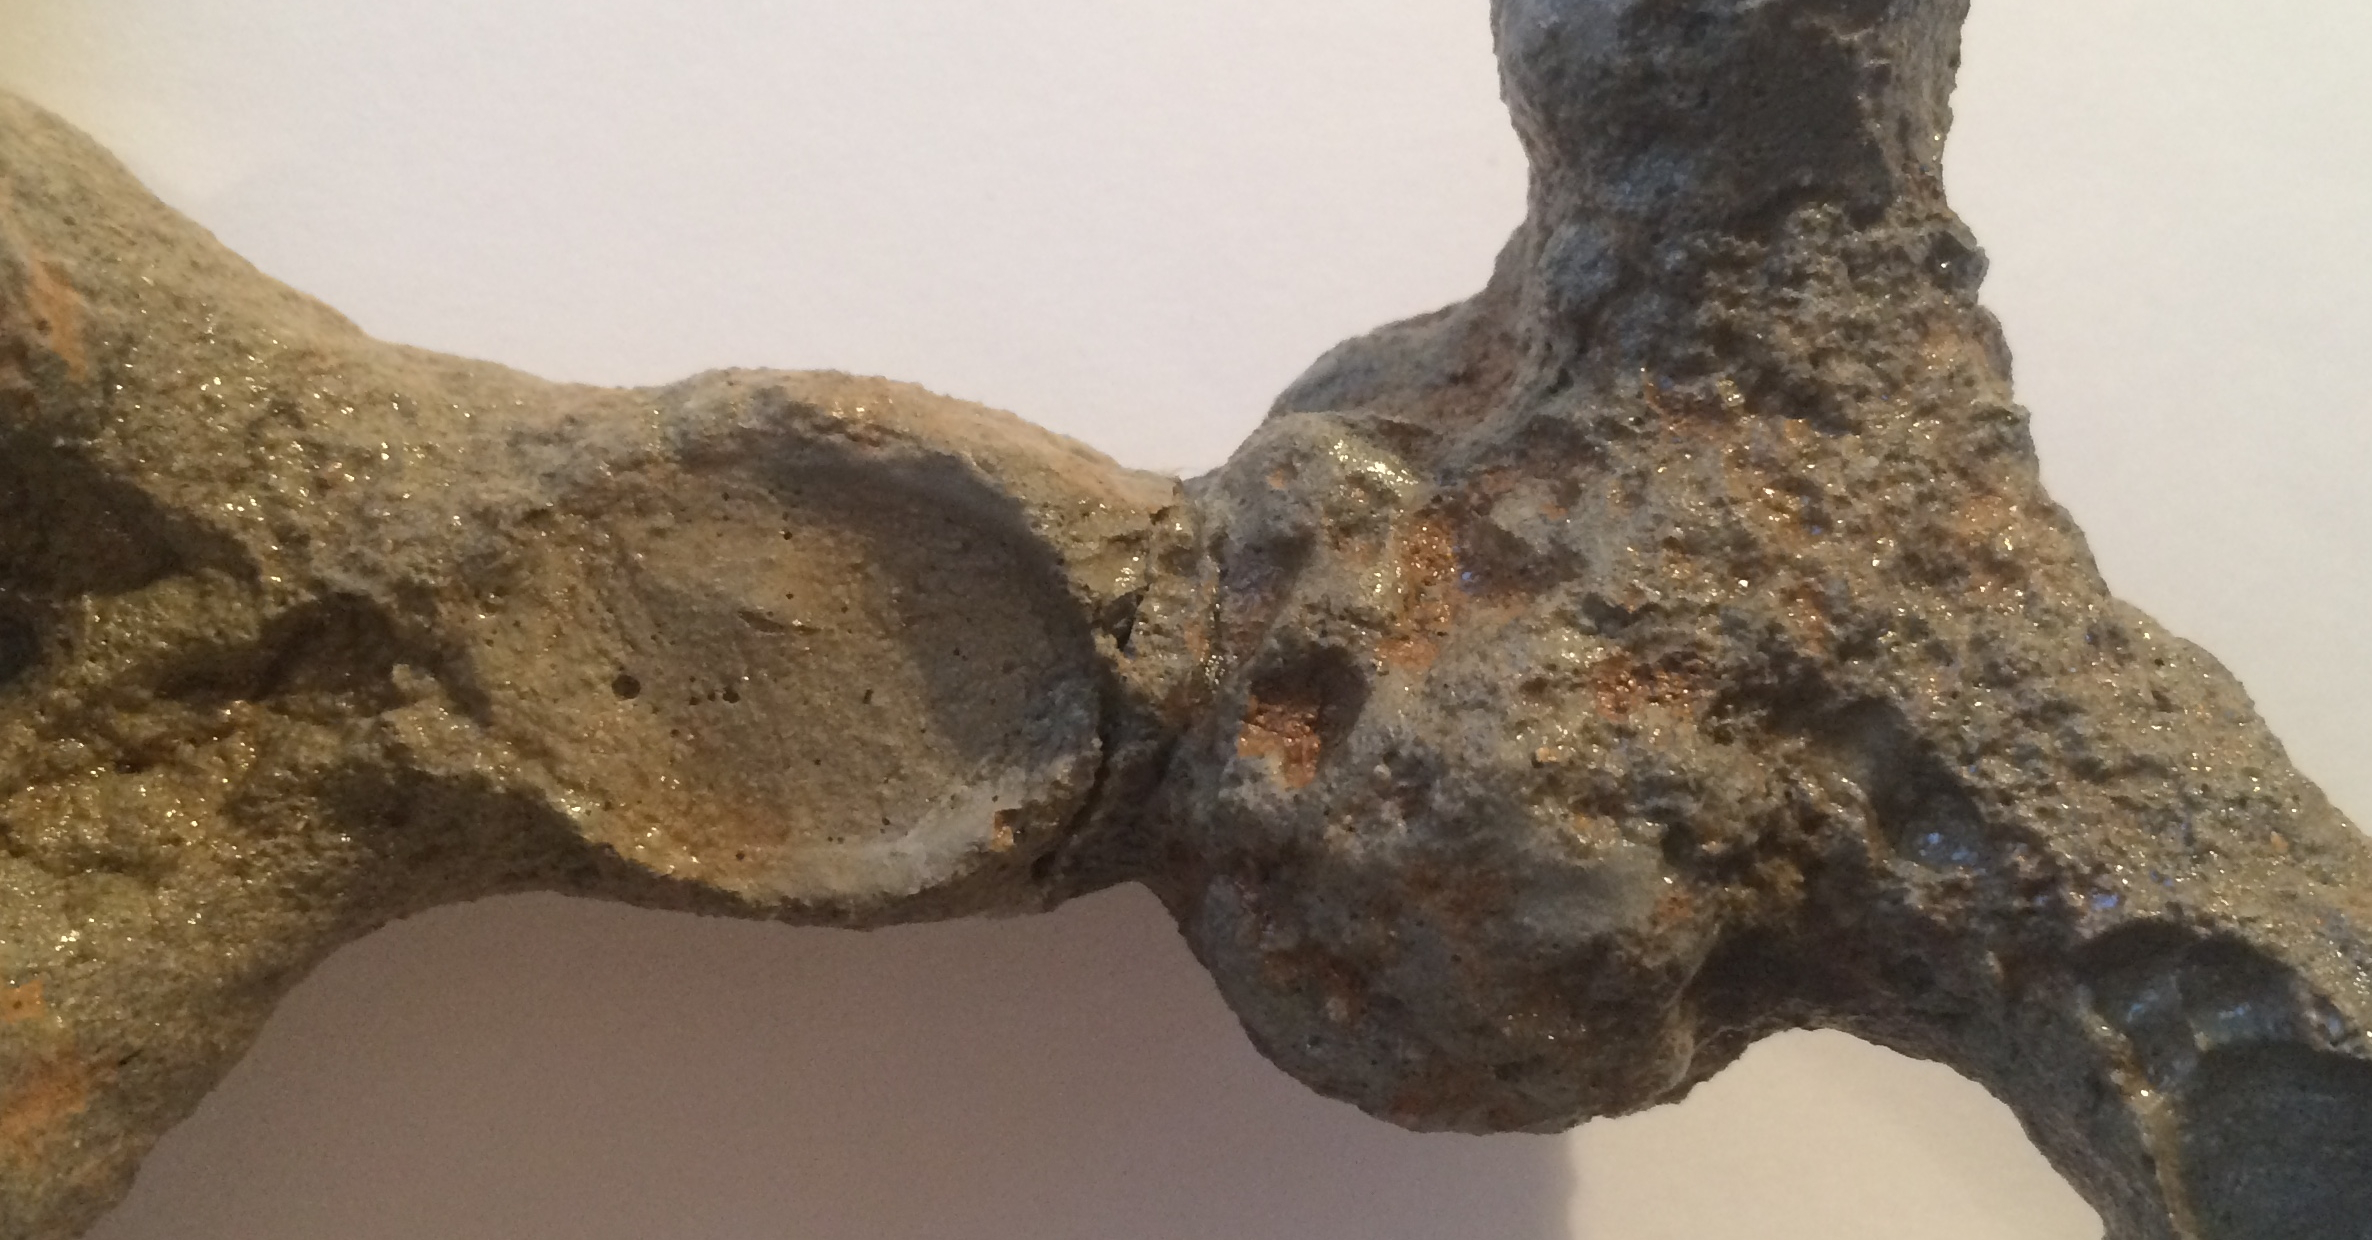
\includegraphics[width=\textwidth]{acoustic_two_exit}
   	\caption{}
   	\label{fig:acoustic_two_exit}
   \end{figure}
   
   \begin{figure}[h]
   	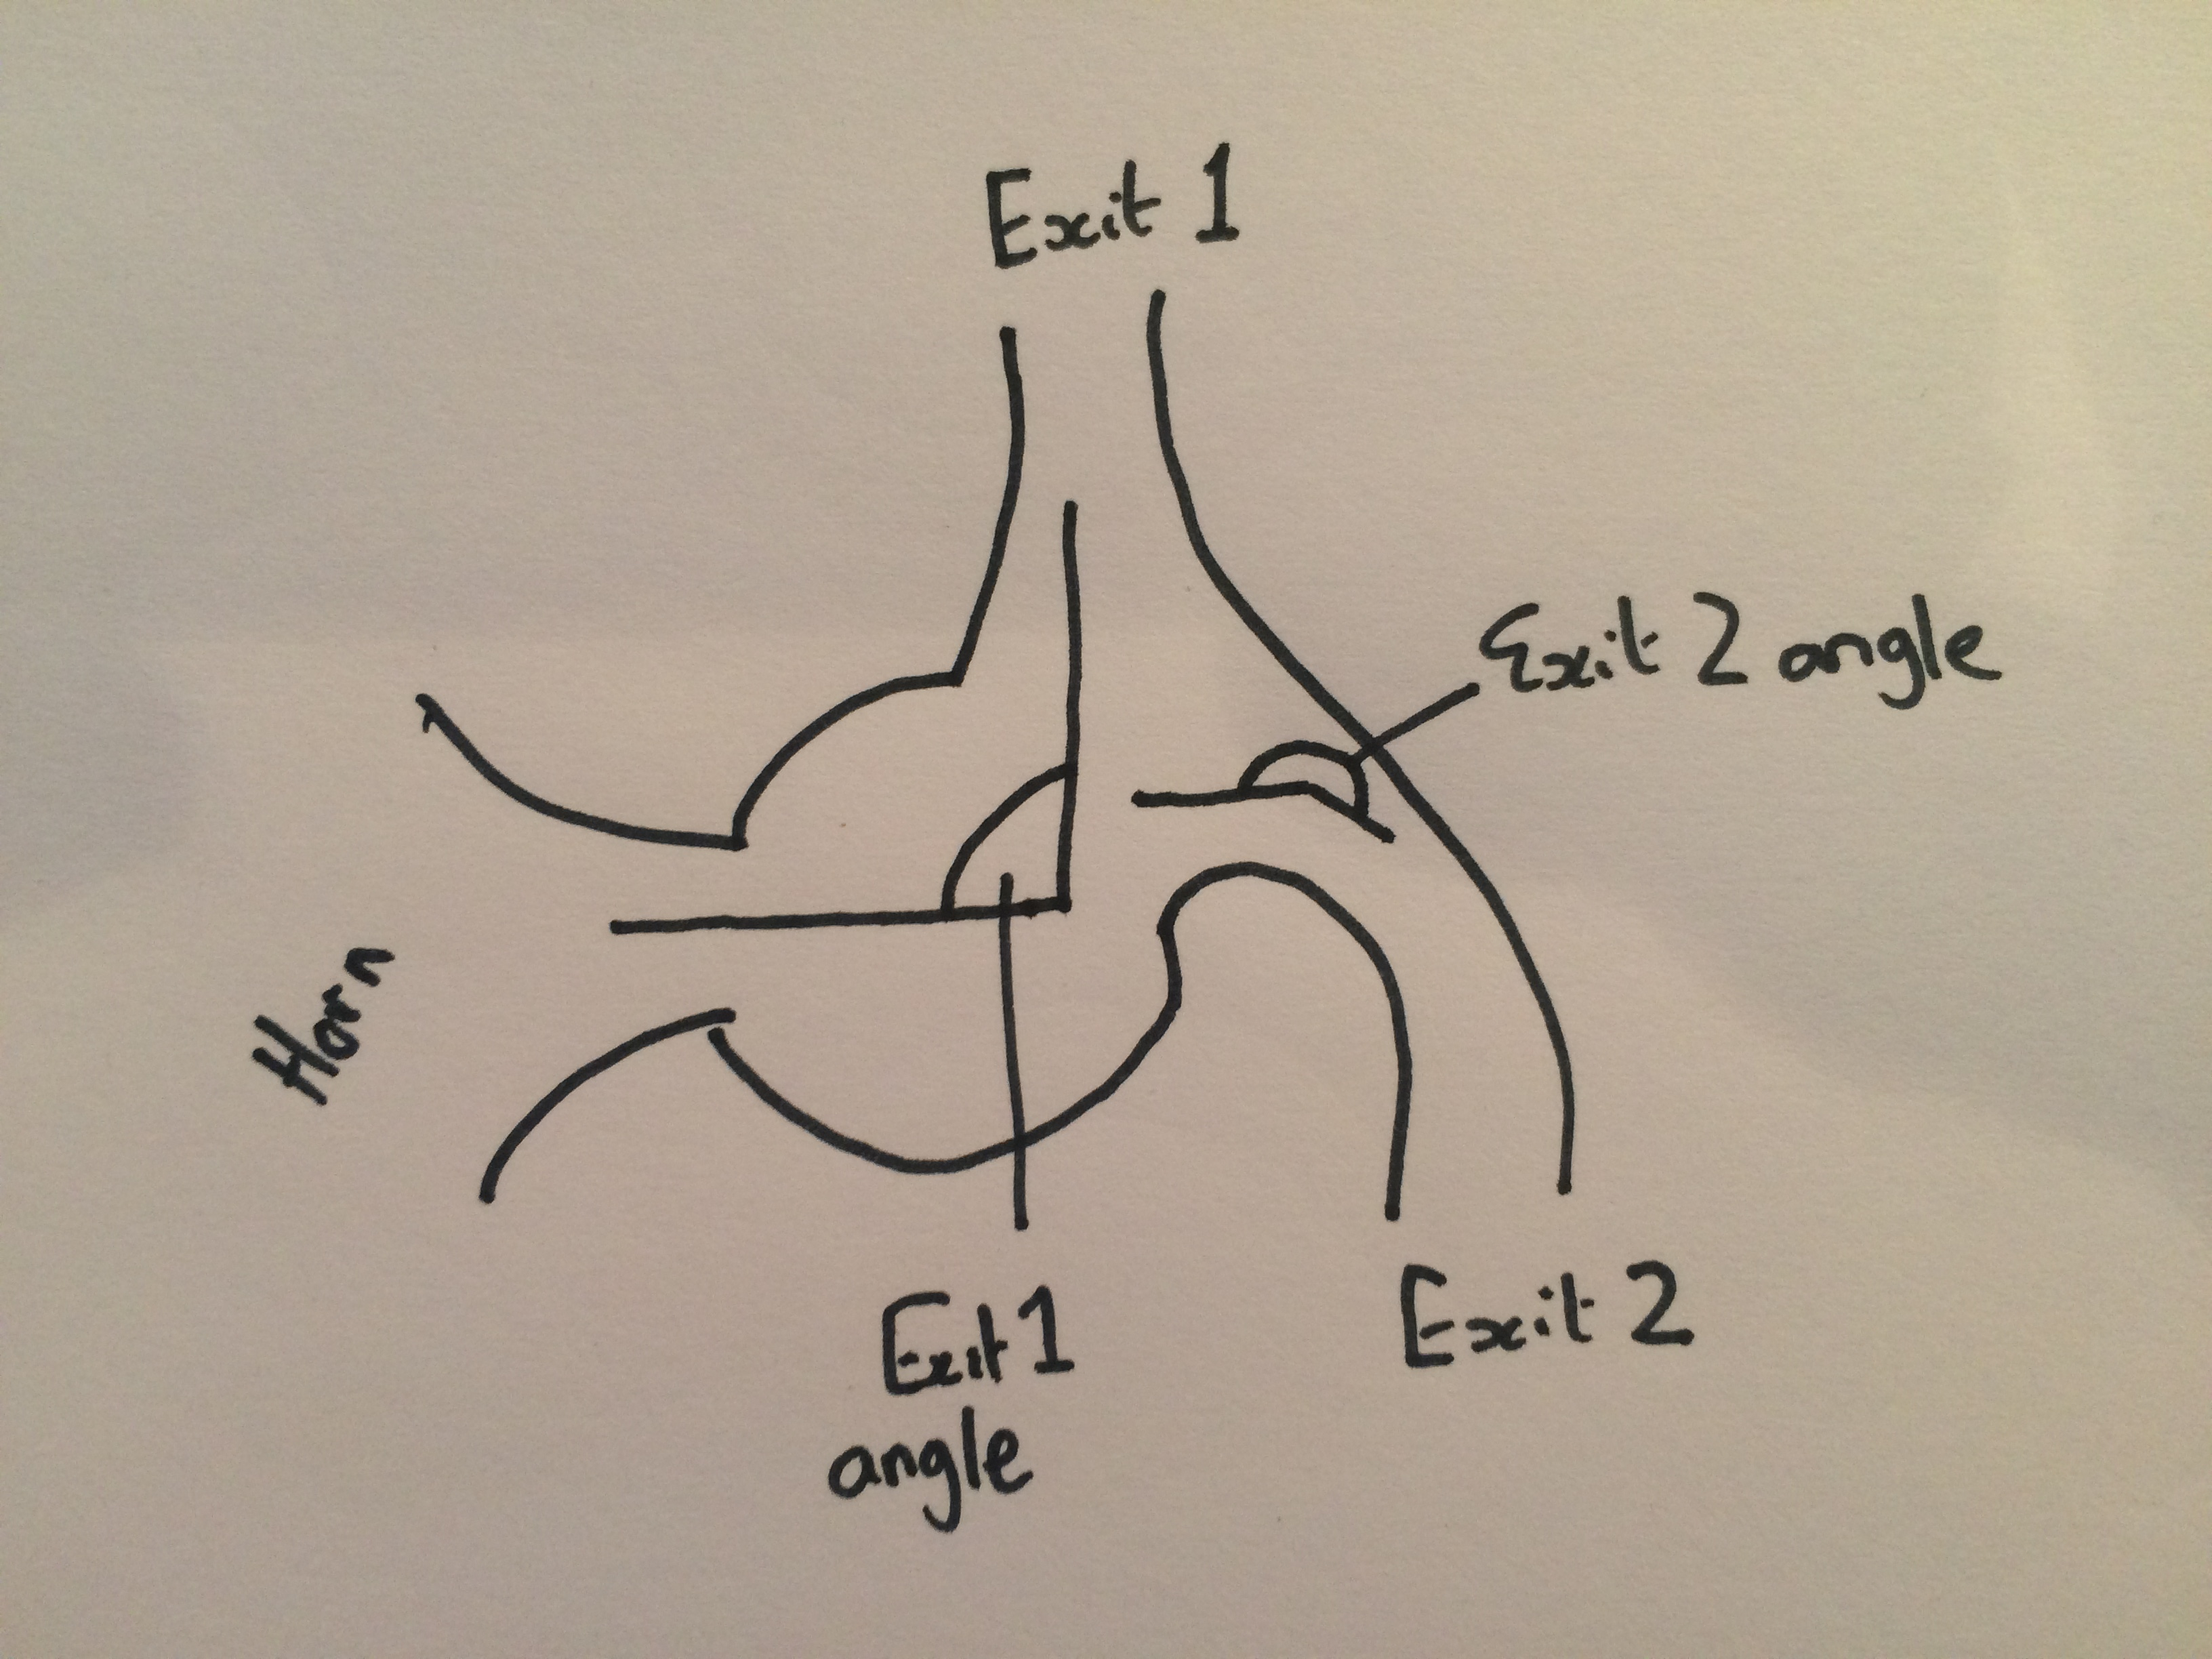
\includegraphics[width=\textwidth]{acoustic_exit_angle}
   	\caption{}
   	\label{fig:acoustic_exit_angle}
   \end{figure}
   
   \section{The burrows of \textit{Gryllotalpa} Latreille, 1802}
   
   \subsection{\textit{Gryllotalpa africana} Palisot de Beauvois, 1805 \cite{palisot1805}}
   The burrows of this species cause damage to turfgrass and crops \cite{brandenburg2002}. Brandenburg et al \cite{brandenburg2002} report the species from heavy clay soil in South Africa. Typical living burrows are Y-shaped (figured in \cite{brandenburg2002}).
   
   \subsection{\textit{Gryllotalpa australis} Erichson, 1842 \cite{erichson1842}}
   The acoustic burrow of this species (figured in \cite{kavanagh1989}) has four exponential horns, with the anterior horns being smaller and more closed placed than the posterior horns. The front horns are sometimes, particularly in shallower soil, fused with the rear horns. The exit tunnel may link to an extensive living burrow system \cite{kavanagh1989}.
   
   \subsection{\textit{Gryllotalpa gryllotalpa} (Linnaeus, 1758) \cite{linnaeus1758}}
   \textit{Gryllus gryllotalpa} Linnaeus, 1758
   \paragraph{}
   The acoustic burrow of this species has between one and six horns arranged in a single line. Single horn acoustic burrow structures in Iran are discussed by \cite{jafari2015}. Bennet-Clark \cite{bennetclark1970a} reports the burrow as generally being double horned with up to six openings. A burrow cast in the NHM collection (NHMUK010211142) appears to have three horns. A 3D scan of the three-horned acoustic burrow cast held by the Natural History Museum, London is described in \cite{baker2016}. Bennet-Clark \cite{bennetclark1970a} states, and the burrow cast he donated ot the NHM agrees with this, that the burrow structure is somewhat irregular. The difference in regularity between Bennet-Clark's casts of \textit{gryllotalpa} and \textit{vineae} is striking (FIG).
   
   \subsection{\textit{Gryllotalpa major} Saussure, 1874 \cite{saussure1874}}
   Walker and Figg \cite{walker1990} describe the song and burrow. Variation in the burrow mouth morphology is discussed by \cite{hill2006}.
   
   \subsection{\textit{Gryllotalpa orientalis} Burmeister, 1838 \cite{burmesietr1838}}
   Living burrows range from a single shallow horizontal burrow to of a network of branching horizontal burrows, with or without one or more vertical burrows \cite{endo2007,endo2008}.
   
   \subsection{\textit{Gryllotalpa vineae} Bennet-Clark, 1970 \cite{bennetclark1970b}}
   The usual form of the acoustic burrow has two horns, although on irregular terrain they may have three or more \cite{bennetclark1970a}. A 3D scan of an acoustic burrow cast held by the Natural History Museum, London is described in \cite{baker2016}. The burrow structure seems to be much more regular, and smoother, than the burrow of \textit{gryllotalpa}.

   \section{The burrows of \textit{Neoscapteriscus} Cadena-Castañeda, 2015}
   Unlike \textit{Gryllotalpa} several species of \textit{Neoscapteriscus} are known to plug their acoustic burrows with soil when not in use \cite{walker1990}.
   
   \paragraph{Taxonomic Note}
   The genus \textit{Neoscapteriscus} contains a number of species previously in the genus \textit{Scapteriscus}. The nomnclature has been updated following the Orthoptera Species File \cite{eades2016}.
   
   \subsection{\textit{Neoscaperiscus borellii} (Giglio-Tos, 1894) \cite{giglio-tos1894}}
   \textit{Scaperiscus borellii} Giglio-Tos, 1894\\
   = \textit{Scapteriscus acletus} Rehn \& Hebard, 1916
   \paragraph{}
   The burrows of this species are known to damage turfgrass on sandy loam soil in the  southeastern USA. The species is mainly herbivorous \cite{brandenburg2002}. Typical living  burrows are Y-shaped with two entrances (figured in \cite{brandenburg2002}).
   \paragraph{}
   Acoustic burrows have a single horn and a turn-around.
   
   \subsection{\textit{Neoscaperiscus vicinus} (Scudder, 1869) \cite{scudder1869}}
   \textit{Neoscaperiscus vicinus} Scudder, 1869
   \paragraph{}
   The burrows of this species are known to damage turfgrass on sandy loam soil in the southeastern USA. The species is mainly carnivorous \cite{brandenburg2002}. Typical living burrows have a single entrance and are branched (figured in \cite{brandenburg2002}).
   \paragraph{}
   Acoustic burrows have a single horn and a turn-around.
   
   \section{Burrow casts held at the Natural History Museum, London}
   The Natural History Museum has a small collection of five mole cricket burrow casts (Table ~\ref{tab:nhm_material}). Measurements of these casts are also provided (Table ~\ref{tab:measurements}).
   
   \paragraph{}
   The first burrow casts presented to the museum were burrow casts of \textit{Gryllotalpa gryllotalpa} and \textit{Gryllotalpa vineae} by H. C. Bennet-Clark in YEAR. \textit{Gryllotalpa vineae} was described in 1970 \cite{bennetclark1970b} by the collector. Although the cast of \textit{vineae} is labelled as being a 'type burrow cast' it does not form part of the type series.
   
   \paragraph{}
   A later donation of three burrow casts was made by Professor David Pye, which show a striking similarity to the double horned burrow of \textit{Gryllotalpa vineae}. As the burrows of mole crickets appear to be closely tuned to the song of the crickets themselves \cite{bennetclark1987,daws1996} and there is variation in the dominant frequency of song between species, it seems probably that identification of species is possible from burrow casts.
   
   \paragraph{}
   Measurements of the burrows held by the NHM, and measurements collected from the scientific literature have been collated in an attempt to determine if species identification from burrows is possible (see below).
   
   
   \subsection{Response to obstructions}
   NHMUK010211181
    
   \begin{landscape}
   \begin{table}[h]
   	\small
	   \begin{tabular}{|l|l|l|l|l|}
		   	\hline  \makecell[l]{Specimen ID\\Accession Number} &
				   	Verbatim ID &
				   	Material &
				   	Notes &
				   	3D Scan URL\\ 
			 \hline	\makecell[l]{NHMUK010211141\\BMNH(E) 1969-431} &
					\textit{G. vineae} &
					Plaster &
					Col. H. C. Bennet-Clark &
					\\
		   	\hline  \makecell[l]{NHMUK010211142 \\ BMNH(E) 1969-431} &
				   	\textit{G. gryllotalpa} &
				   	Plaster &
				   	Col. H. C. Bennet-Clark &
				   	\\
		   	\hline  \makecell[l]{NHMUK010211179 \\ BMNH(E) 2016-33} &
				   	\textit{G. ?vineae} &
					Builders' Cement &
					\makecell[l]{
						Olive grove in Vale de Boa Hora, Algarve, Portugal \\
						25.xii.1974 \\
						Presented by Prof. David Pye
					} &
					\\ 
		   	\hline  \makecell[l]{NHMUK010211180 \\ BMNH(E) 2016-33} &
				   	\textit{G. ?vineae} &
				   	Builders' Cement &
				   	\makecell[l]{
				   		Olive grove in Vale de Boa Hora, Algarve, Portugal \\
				   		25.xii.1974 \\
				   		Presented by Prof. David Pye
				   	} &
				   	\\ 
		   	\hline  \makecell[l]{NHMUK010211171 \\ BMNH(E) 2016-33} &
				   	\textit{G. ?vineae} &
					Builders' Cement &
					\makecell[l]{
						Olive grove in Vale de Boa Hora, Algarve, Portugal \\
						25.xii.1974 \\
						Presented by Prof. David Pye
					} &
					\\  
		   	\hline 
		\end{tabular}
   \caption{Burrow cast specimens held by the Natural History Museum, London}
   \label{tab:nhm_material}
   \end{table}
   \end{landscape}

   \begin{landscape}
   		\thispagestyle{plain}
	   	\begin{table}
	   		\tiny
   		\begin{tabular}{|l|c|c|c|c|c|c|c|c|c|c|c|c|c|c|c|c|}
   			\hline 	Cast &
		   			\makecell{Opening 1\\Length} &
		   			\makecell{Opening 1\\Width} &
		   			\makecell{Opening 2\\Length} &
		   			\makecell{Opening 2\\Width} &
		   			\makecell{Opening 3\\Length} &
		   			\makecell{Opening 3\\Width} &
		   			\makecell{Opening\\Spacing} &
		   			\makecell{Throat\\Height} &
		   			\makecell{Throat\\Width} &
		   			\makecell{Bulb\\Length} & 
		   			\makecell{Bulb\\Height} &
		   			\makecell{Bulb\\Width} &
		   			\makecell{Exit 1\\Height} &
		   			\makecell{Exit 1\\Width} &
		   			\makecell{Exit 2\\Height} &
		   			\makecell{Exit 2\\Width} \\
		   	\hline	NHMUK010211141 &
				   	42 &
				   	25 &
				   	36 &
				   	25 &
				   	&
				   	&
				   	29 &
				   	19 &
				   	16 &
				   	29 &
				   	27 &
				   	29 &
				   	16 &
				   	15 &
				   	&
				   	\\
				   	
			\hline	NHMUK010211142 &
					30 &
					23 &
					20 &
					31 &
					44 &
					26 &
					40 &
					18 &
					34 &
					33 &
					30 &
					17 &
					13 &
					&
					&
					\\
					
		   	\hline	NHMUK010211179 &
				   	35 &
				   	21 &
				   	35 &
				   	23 &
				   	&
				   	&
				   	30 &
				   	24 &
				   	17 &
				   	37 &
				   	34 &
				   	30 &
				   	14 &
				   	15 &&\\
		   	\hline	NHMUK010211180 &
				   	31 &
				   	28 &
				   	40 &
				   	27 &
				   	&
				   	&
				   	28 &
				   	29 &
				   	18 &
				   	32 &
				   	35 &
				   	36 &
				   	17 &
				   	19 &
				   	20 &
				   	21 \\
			\hline	NHMUK010211181 &
					40 &
					19 &
					34 &
					23 &
					&
					&
					29 &
					20 &
					17 &
					27 &
					28 &
					30 &
					17 &
					15 &&\\
			
			\hline
				   	
   		\end{tabular}
   		\caption{Burrow cast measurements of NHM material. All measurements are in mm, to the nearest mm. Measurements were made using Mitutoyo Absolute Digimatic digital calipers.}
   		\label{tab:measurements}
	   	\end{table}
   	\end{landscape}
   	
   \section{Comparison of acoustic burrows between species}
   Table ~\ref{tab:comparisons} gives a comparison of measurements of mole cricket acoustic burrows taken from the literature and from specimens at the Natural History Museum, London (NHMUK).
   \begin{landscape}
   	\thispagestyle{plain}
   	\begin{table}

   		\tiny
   		\begin{tabular}{|l|l|l|l|l|l|l|l|l|l|l|l|l|l|}
   			\hline 	Species &
		   			\makecell{Number of\\Openings} &
		   			\makecell{Opening\\Length} &
		   			\makecell{Opening\\Width} &
		   			\makecell{Opening\\spacing} &
		   			\makecell{Horn\\Length} &
		   			\makecell{Throat\\Height} &
		   			\makecell{Throat\\Width} &
		   			\makecell{Bulb\\Length} &
		   			\makecell{Bulb\\Height} &
		   			\makecell{Bulb\\Width} &
		   			Depth &
		   			\makecell{Exit\\Height} &
		   			\makecell{Exit\\Width} \\
		   	\hline	\makecell{\textit{Gryllotalpa australis}\\from \cite{kavanagh1989}} &
				   	4 &
				   	&
				   	&
				   	&
				   	&
				   	\multicolumn{2}{c|}{$11.5\pm1$} &
				   	$24.3\pm1.5$ &
				   	$22.8\pm3.4$ &
				   	$20.6\pm2.9$ &
				   	&
				   	\multicolumn{2}{c|}{$13.8\pm1.4$} \\
   			\hline  \makecell{\textit{Gryllotalpa gryllotalpa}\\from \cite{jafari2015}} &
		   			1 &
		   			$32.6\pm1.86$ &
		   			$42.8\pm1.69$ & 
		   			&
		   			\makecell{$45.2\pm2.13$\\but see text} &
		   			$21.2\pm0.59$ &
		   			$20\pm0.83$ &
		   			$28\pm2.13$ &
		   			$22.8\pm2.01$ &
		   			$25\pm2.03$ &
		   			&
		   			$18\pm0.07$ &
		   			$20\pm0.04$ \\ 
   			\hline	\makecell{\textit{Gryllotalpa major}\\from \cite{walker1990}} &
		   			1 &
		   			$26\pm1.2$ &
		   			$86\pm4.4$ &
		   			&
		   			$64\pm2.0$ &
		   			$19\pm0.7$ &
		   			$14\pm0.6$ &
		   			$39\pm0.8$ &
		   			$33\pm1.2$ &
		   			$37\pm1.4$ &
		   			$19\pm5$ &
		   			$14\pm0.4$ &
		   			$14\pm0.5$ \\
		   	\hline 	\makecell{\textit{Neoscapteriscus borellii}\\from \cite{nickerson1979}} &
				   	1 &
				   	&
				   	&
				   	&
				   	&
				   	\multicolumn{2}{c|}{$12\pm1$} &
				   	$19\pm4$ &
				   	$15\pm1$ &
				   	$14\pm2$ &
				   	&
				   	\multicolumn{2}{c|}{$12\pm1$} \\
			\hline 	\makecell{\textit{Neoscapteriscus vicinus}\\from \cite{nickerson1979}} &
					1 &
					&
					&
					&
					&
					\multicolumn{2}{c|}{$13\pm1$} &
					$19\pm1$ &
					$16\pm1$ &
					$14\pm1$ &
					&
					\multicolumn{2}{c|}{$12\pm1$} \\	
   			\hline
   		
   		\end{tabular} 
   		\caption{Comparison of measurements of acoustic burrows between different species, compiled from literature and the NHM collection.}
   		\label{tab:comparisons}
   	\end{table}
   \end{landscape}
   \subsection{Eccentricity}
   The eccentricity of an ellipse is a quantitative measure of how much that ellipse deviates from a perfect circle. A circle has an eccentricity of 0, while an ellipse that has been so greatly deformed from a circle that is essentially a line has an eccentricity of 1.
   
   \paragraph{}
   Since the eccentricity of an ellipse is independent of its orientation, we must specify the orientation of the ellipse relative to the burrow. This is easiest achieved by specifying the direction of the major axis (length, width, height).
   
   \paragraph{}
   The eccentricity of a burrow is a measure of shape, rather than size, so accounts for size between the burrows of individuals of varying size within a single species.
      
   \subsection{Calculation of eccentricity}
   The calculation path here is used as measuring the length of the major axis (L) and minor axis (l) is straightforward for a burrow. The major axis is the longest measurement of opening length or opening width, with the other measurement becoming the minor axis (FIG). The calculation of the distance between the centre of the ellipse and one of the foci is calculated as follows.
   
   \[
      Major\ radius:\ M = \frac{L}{2}
   \]
   
   \[
     Minor\ radius:\ m = \frac{l}{2}
   \]
   
   \[
     Focal\ distance: F = \sqrt{M^2 - m^2}
   \]
   
   \begin{equation}
     Eccentricity:\ e = \frac{F}{a} = \frac{F}{\sqrt{F^2+m^2}}
     \label{eq:eellipse_eccentricity}
   \end{equation}
   
   Examples of varying eccentricity is given in Figure ~\ref{fig:eccentricity_examples}.
   
   \begin{figure}
   	\tikz \draw (0,0) ellipse (1cm and 1cm);
   	\tikz \draw (0,0) ellipse (1.25cm and 1cm);
   	\tikz \draw (0,0) ellipse (1.5cm and 1cm);
   	\tikz \draw (0,0) ellipse (2cm and 1cm);
   	\caption{Ellipses with eccentricity of (left to right) 0, 0.6, 0.75 \& 0.87}
   	\label{fig:eccentricity_examples}
   \end{figure}
   
   \subsection{Constriction eccentricity}
   As previously noted, there has been variation in the published literature as to whether to estimate a single diameter for the two constrictions, or measure both height and width. The shape of the constriction will be influenced by the shape of either the horn or exit tunnel it attaches to the bulb.
   
   \subsubsection{Throat eccentricity} Table ~\ref{tab:throat_eccentricity} shows throat eccentricities.
   
   \subsubsection{Exit eccentricity} Table ~\ref{tab:exit_eccentricity} shows exit eccentricities. 
   
   
   TODO: Add note on height/width or diameter measurement previously.
   
      \begin{table}[h]
      	\begin{tabular}{|l|c|c|}
      		\hline 	Species &
		      		Plane of Eccentricity &
		      		Eccentricity \\ 
      		\hline  \textit{Gryllotalpa gryllotalpa} from \cite{jafari2015} &
		      		high &
		      		0.33  \\
      		\hline	\textit{Gryllotalpa major} from \cite{walker1990} &
		      		high &
		      		0.68 \\
		    \hline	\textit{Gryllotalpa vineae} NHM Bennett-Clark &
				    high &
					0.54 \\
      		\hline 
      	\end{tabular}
      	\caption{Throat eccentricities of mole cricket burrows.}
      	\label{tab:throat_eccentricity}
      \end{table} 
      
      \begin{table}[h]
      	\begin{tabular}{|l|c|c|}
      		\hline 	Species &
	      		Plane of Eccentricity &
	      		Eccentricity \\ 
      		\hline  \textit{Gryllotalpa gryllotalpa} from \cite{jafari2015} &
	      		wide &
	      		0.44  \\
      		\hline	\textit{Gryllotalpa major} from \cite{walker1990} &
	      		&
	      		0 \\
	      	\hline	\textit{Gryllotalpa vineae} NHM Bennet-Clark &
		      	high &
		      	0.35 \\
      		\hline 
      	\end{tabular}
      	\caption{Exit eccentricities of mole cricket burrows.}
      	\label{tab:exit_eccentricity}
      \end{table} 
   
   \subsection{Horn opening eccentricity}
   The eccentricity of the horn openings for species with data available in Table ~\ref{tab:comparisons} are given in Table ~\ref{tab:horn_eccentricity}.
   \begin{table}[h]
   \begin{tabular}{|l|c|c|}
   	\hline 	Species &
		   	Plane of Eccentricity &
		   	Eccentricity \\ 
   	\hline  \textit{Gryllotalpa gryllotalpa} from \cite{jafari2015} &
		   	wide &
		   	$0.65\pm0.08$  \\
	\hline	\textit{Gryllotalpa major} from \cite{walker1990} &
			wide &
			$0.95\pm0.01$ \\
	\hline \textit{Gryllotalpa vineae} NHM Bennett-Clark &
			long &
			$0.76\pm0.04$ \\
	\hline	\textit{Gryllotalpa gryllotalpa} NHM Bennett-Clark &
			either &
			variable (0.64-0.81) \\
	
   	\hline 
   \end{tabular}
   \caption{Acoustic horn eccentricities of mole cricket species.}
   \label{tab:horn_eccentricity}
   \end{table} 
   
   \subsection{The identity of NHMUK010211179-81}
   The horn eccentricity of these (assumed conspecific) casts were calculated as $0.72\pm0.14$ in the length direction. It can be seen from Table ~\ref{tab:horn_eccentricity} that the only species that overlaps in horn opening shape is \textit{Gryllotalpa vineae}. Further comparisons are given in Table ~\ref{tab:id_nhm_casts}.
   
   \paragraph{}
   It can be seen (Figure ~\ref{fig:radar_eccentricity})  there is close agreement between the three more recent specimens and the Bennett-Clark specimen confirmed to be \textit{vineae}. Given that only a single confirmed specimen of \textit{vineae} for comparison, it is likely that the three newer casts fall within the normal bacoustic burrow range of that species. They appear distinct from other species of \textit{Gryllotalpa} on factors including number of horns and horn opening eccentricity. As shown by Bennet-Clark the shape of the exit tunnel has little effect on the burrow acoustics, so there is less evolutionary pressure to maintain a uniform shape ofthis section between burrows. In addition the species varies from the NHM \textit{G. gryllotalpa} cast by its regular and smooth structure.
   
      \begin{figure}[h]
      	\includegraphics[width=\textwidth]{radar_eccentricity}
      	\caption{Radar plot of eccentricity measurements of mole cricket burrows. Eccentricities along the anterior-posterior axis are given positive values, those orthogonal to it are given negative values.}
      	\label{fig:radar_eccentricity}
      \end{figure}
      
   
   \subsection{\textit{Gryllotalpa gryllotalpa}: highly variable?}
   There is a striking difference between the cast of this species donated by Bennett-Clark to the NHM and the Iranian specimens examined by \cite{jafari2015}. This species is known to have multiple races across Europe, and it is possible that acoustic burrow structure also varies considerably across this range.
   
   \begin{table}[h]
   	\begin{tabular}{|l|c|c|}
   		\hline 	Measurement &
		   		NHMUK010211179-81 &
		   		\makecell{\textit{Gryllotalpa vineae}\\NHM Bennett-Clark} \\ 
   		\hline  Horn opening eccentricity &
		   		length $0.72\pm0.14$ &
		   		length $0.76\pm0.04$  \\
   		\hline	Throat eccentricity &
		   		height $0.67\pm0.10$ &
		   		height 0.54 \\
   		\hline  Exit eccentricity &
		   		various 0.43 &
			   	height 0.35 \\
   		
   		\hline 
   	\end{tabular}
   	\caption{Comparison of measurements of NHMUK010211179-81 with \textit{Gryllotalpa vineae}.}
   	\label{tab:id_nhm_casts}
   \end{table}
   
   \section{Acknowledgements}
   Thanks to George Beccaloni and Judith Marshall (Natural History Museum, London).
   \printbibliography{}
\end{document}